\chapter{Mô Tả Thiết Kế Phần Mềm}

\section{Thiết Kế Hệ Thống}

\subsection{Kiến Trúc Hệ Thống}

Hệ thống \texttt{SmartDroneDelivery} được xây dựng theo mô hình kiến trúc đa tầng (Multi-tier Architecture) nhằm tách biệt các trách nhiệm và nâng cao khả năng bảo trì, nâng cấp phần mềm. Kiến trúc hệ thống bao gồm ba tầng chính như sau:

\begin{enumerate}[leftmargin=*]
  \item \textbf{Tầng Giao Diện (Presentation Layer / Client):}
    \begin{itemize}
      \item \textbf{Customer Web Portal (React):} Ứng dụng Web dành cho Khách hàng giao tiếp qua trình duyệt để gửi yêu cầu đặt hàng mới, nhận thông báo điện tử, định vị hành trình bay của drone thời gian thực và trò chuyện trực tiếp với Trợ lý ảo (Chatbot AI).
      \item \textbf{Management Web Portal (React):} Ứng dụng Web quản lý dành cho nhà nội bộ gồm Quản lý Logistics, Điều phối viên (Dispatcher) và Nhân viên trạm (Station Operator). Hỗ trợ duyệt hàng, lập lịch bay, quản lý vận hành trạm và thiết bị drone, xử lý sự cố phát sinh.
      \item Hai ứng dụng Web trên liên kết với tầng Backend thông qua giao thức HTTP/HTTPS (REST API) và WebSockets (truyền tọa độ trực tuyến).
    \end{itemize}
  \item \textbf{Tầng Nghiệp Vụ (Application Layer / Backend REST API):}
    \begin{itemize}
      \item Được phát triển dựa trên ngôn ngữ \textbf{Python} và khung ứng dụng \textbf{Flask}.
      \item Flask tiếp nhận các yêu cầu REST API, thực hiện kiểm lỗi, và kiểm soát các ràng buộc nghiệp vụ (giới hạn tải trọng 5kg, chặn sửa đổi đơn sau khi duyệt).
      \item Tầng Backend còn tích hợp dịch vụ phụ trợ như \textbf{LLM API (Groq/Gemini)} thông qua giao thức HTTPS để vận hành trợ lý chatbot AI đàm thoại với khách hàng.
    \end{itemize}
  \item \textbf{Tầng Dữ Liệu (Data Layer / Database Store):}
    \begin{itemize}
      \item Sử dụng hệ quản trị cơ sở dữ liệu quan hệ \textbf{PostgreSQL} (chạy trên dịch vụ Cloud Supabase).
      \item Mối liên kết giữa \textbf{Flask Backend} và \textbf{PostgreSQL Database} được thực hiện thông qua kết nối mạng \textbf{TCP/IP} (Transmission Control Protocol) bằng thư viện SQLAlchemy ORM trên cổng kết nối mặc định \texttt{5432}. Tất cả các truy vấn dữ liệu và giao dịch (transaction) được mã hóa bảo mật thông qua giao thức TCP.
    \end{itemize}
\end{enumerate}

\begin{figure}[H]
  \centering
  \includegraphics[width=0.9\textwidth]{so-do/diagrams/arch_backend.png}
  \caption{Sơ đồ cấu trúc phân tầng Flask Backend của SmartDroneDelivery}
  \label{fig:arch-backend}
\end{figure}

\subsection{Sơ Đồ Package}

\section{Thiết Kế Cơ Sở Dữ Liệu}

\subsection{Sơ Đồ Thực Thể Quan Hệ}

\begin{figure}[H]
  \centering
  
\includegraphics[width=\textwidth]{so-do/ERD.pdf}
  \caption{Sơ đồ thực thể quan hệ của hệ thống SmartDroneDelivery}
  \label{fig:erd}
\end{figure}

\subsection{Mô Tả Chi Tiết Các Bảng}

\begin{table}[H]
  \centering
  \begin{tabularx}{\textwidth}{|l|l|l|>{\raggedright\arraybackslash}X|}
    \hline
    \textbf{Tên cột} & \textbf{Kiểu dữ liệu} & \textbf{Ràng buộc} & \textbf{Mô tả} \\
    \hline
    ma\_vai\_tro         & UUID            & PK, NOT NULL    & Mã vai trò (tự động tạo UUID) \\ \hline
    ten\_vai\_tro        & VARCHAR(50)     & NOT NULL, UNIQUE & Tên vai trò (Admin, Dispatcher, v.v.) \\ \hline
    created\_at          & TIMESTAMPTZ     & NOT NULL        & Thời gian tạo bản ghi \\ \hline
    updated\_at          & TIMESTAMPTZ     & NOT NULL        & Thời gian cập nhật bản ghi \\
    \hline
  \end{tabularx}
  \caption{Cấu trúc bảng \texttt{vai\_tro} (Vai trò người dùng)}
  \label{tab:db-vai-tro}
\end{table}

\begin{table}[H]
  \centering
  \begin{tabularx}{\textwidth}{|l|l|l|>{\raggedright\arraybackslash}X|}
    \hline
    \textbf{Tên cột} & \textbf{Kiểu dữ liệu} & \textbf{Ràng buộc} & \textbf{Mô tả} \\
    \hline
    ma\_nguoi\_dung      & UUID            & PK, NOT NULL    & Mã người dùng (tự động tạo UUID) \\ \hline
    ma\_vai\_tro         & UUID            & FK, NOT NULL    & Khóa ngoại tham chiếu đến bảng vai\_tro \\ \hline
    ho\_ten              & VARCHAR(150)    & NOT NULL        & Họ và tên người dùng \\ \hline
    email                & VARCHAR(255)    & NOT NULL, UNIQUE & Địa chỉ email người dùng \\ \hline
    so\_dien\_thoai      & VARCHAR(20)     & NULL            & Số điện thoại liên hệ \\ \hline
    mat\_khau\_hash      & TEXT            & NOT NULL        & Mật khẩu đã mã hóa hash \\ \hline
    ngay\_tao            & TIMESTAMPTZ     & NOT NULL        & Ngày giờ tạo tài khoản \\ \hline
    updated\_at          & TIMESTAMPTZ     & NOT NULL        & Thời gian cập nhật gần nhất \\
    \hline
  \end{tabularx}
  \caption{Cấu trúc bảng \texttt{nguoi\_dung} (Tài khoản người dùng)}
  \label{tab:db-nguoi-dung}
\end{table}

\begin{table}[H]
  \centering
  \begin{tabularx}{\textwidth}{|l|l|l|>{\raggedright\arraybackslash}X|}
    \hline
    \textbf{Tên cột} & \textbf{Kiểu dữ liệu} & \textbf{Ràng buộc} & \textbf{Mô tả} \\
    \hline
    ma\_kh               & UUID            & PK, NOT NULL    & Mã khách hàng (tự động tạo UUID) \\ \hline
    ten                  & VARCHAR(50)     & NOT NULL        & Tên khách hàng \\ \hline
    ten\_dem             & VARCHAR(50)     & NULL            & Tên đệm \\ \hline
    ho                   & VARCHAR(50)     & NOT NULL        & Họ của khách hàng \\ \hline
    gioi\_tinh           & VARCHAR(10)     & CHECK           & Giới tính (Nam, Nữ, Khác) \\ \hline
    so\_dien\_thoai      & VARCHAR(20)     & NULL            & Số điện thoại liên hệ \\ \hline
    email                & VARCHAR(255)    & UNIQUE          & Địa chỉ email khách hàng \\ \hline
    ngay\_sinh           & DATE            & NULL            & Ngày tháng năm sinh \\ \hline
    created\_at          & TIMESTAMPTZ     & NOT NULL        & Thời gian tạo bản ghi \\ \hline
    updated\_at          & TIMESTAMPTZ     & NOT NULL        & Thời gian cập nhật bản ghi \\
    \hline
  \end{tabularx}
  \caption{Cấu trúc bảng \texttt{khach\_hang} (Thông tin khách hàng)}
  \label{tab:db-khach-hang}
\end{table}

\begin{table}[H]
  \centering
  \begin{tabularx}{\textwidth}{|l|l|l|>{\raggedright\arraybackslash}X|}
    \hline
    \textbf{Tên cột} & \textbf{Kiểu dữ liệu} & \textbf{Ràng buộc} & \textbf{Mô tả} \\
    \hline
    ma\_dia\_chi         & UUID            & PK, NOT NULL    & Mã địa chỉ (tự động tạo UUID) \\ \hline
    ma\_kh               & UUID            & FK, NOT NULL    & Khóa ngoại tham chiếu đến bảng khach\_hang \\ \hline
    dia\_chi\_cu\_the    & TEXT            & NOT NULL        & Địa chỉ chi tiết (số nhà, tên đường) \\ \hline
    thanh\_pho           & VARCHAR(100)    & NOT NULL        & Tên tỉnh hoặc thành phố \\ \hline
    lat                  & DOUBLE          & NOT NULL        & Vĩ độ GPS trên bản đồ \\ \hline
    lng                  & DOUBLE          & NOT NULL        & Kinh độ GPS trên bản đồ \\ \hline
    created\_at          & TIMESTAMPTZ     & NOT NULL        & Thời gian tạo bản ghi \\ \hline
    updated\_at          & TIMESTAMPTZ     & NOT NULL        & Thời gian cập nhật bản ghi \\
    \hline
  \end{tabularx}
  \caption{Cấu trúc bảng \texttt{dia\_chi} (Địa chỉ giao hàng)}
  \label{tab:db-dia-chi}
\end{table}

\begin{table}[H]
  \centering
  \begin{tabularx}{\textwidth}{|l|l|l|>{\raggedright\arraybackslash}X|}
    \hline
    \textbf{Tên cột} & \textbf{Kiểu dữ liệu} & \textbf{Ràng buộc} & \textbf{Mô tả} \\
    \hline
    ma\_tin\_nhan        & UUID            & PK, NOT NULL    & Mã tin nhắn (tự động tạo UUID) \\ \hline
    ma\_kh               & UUID            & FK, NOT NULL    & Khóa ngoại tham chiếu đến bảng khach\_hang \\ \hline
    noi\_dung            & TEXT            & NOT NULL        & Nội dung tin nhắn khách hàng gửi \\ \hline
    phan\_hoi            & TEXT            & NULL            & Nội dung phản hồi từ Chatbot AI \\ \hline
    thoi\_gian           & TIMESTAMPTZ     & NOT NULL        & Thời gian gửi tin nhắn \\
    \hline
  \end{tabularx}
  \caption{Cấu trúc bảng \texttt{tin\_nhan\_chatbot} (Lịch sử chat AI)}
  \label{tab:db-tin-nhan-chatbot}
\end{table}

\begin{table}[H]
  \centering
  \begin{tabularx}{\textwidth}{|l|l|l|>{\raggedright\arraybackslash}X|}
    \hline
    \textbf{Tên cột} & \textbf{Kiểu dữ liệu} & \textbf{Ràng buộc} & \textbf{Mô tả} \\
    \hline
    ma\_don\_hang        & UUID            & PK, NOT NULL    & Mã đơn hàng (tự động tạo UUID) \\ \hline
    ma\_kh               & UUID            & FK, NOT NULL    & Khóa ngoại tham chiếu đến bảng khach\_hang \\ \hline
    ma\_dia\_chi         & UUID            & FK, NOT NULL    & Khóa ngoại tham chiếu đến bảng dia\_chi \\ \hline
    trang\_thai\_don\_hang & VARCHAR(30)     & NOT NULL, CHECK & Trạng thái đơn (Chờ duyệt, Đã duyệt, Đang giao, v.v.) \\ \hline
    cach\_thuc\_thanh\_toan & VARCHAR(50)     & NULL            & Phương thức thanh toán \\ \hline
    tong\_tien           & DECIMAL(15,2)   & DEFAULT 0       & Tổng giá trị đơn hàng \\ \hline
    ngay\_dat\_hang      & TIMESTAMPTZ     & NOT NULL        & Ngày giờ đặt đơn hàng \\ \hline
    ngay\_cap\_nhat      & TIMESTAMPTZ     & NOT NULL        & Thời gian cập nhật gần nhất \\
    \hline
  \end{tabularx}
  \caption{Cấu trúc bảng \texttt{don\_hang} (Đơn hàng giao)}
  \label{tab:db-don-hang}
\end{table}

\begin{table}[H]
  \centering
  \begin{tabularx}{\textwidth}{|l|l|l|>{\raggedright\arraybackslash}X|}
    \hline
    \textbf{Tên cột} & \textbf{Kiểu dữ liệu} & \textbf{Ràng buộc} & \textbf{Mô tả} \\
    \hline
    ma\_tram             & UUID            & PK, NOT NULL    & Mã trạm hạ cánh (tự động tạo UUID) \\ \hline
    ten\_tram            & VARCHAR(150)    & NOT NULL        & Tên trạm hạ cánh \\ \hline
    dia\_chi\_tram       & TEXT            & NOT NULL        & Địa chỉ chi tiết của trạm \\ \hline
    lat                  & DOUBLE          & NOT NULL        & Vĩ độ GPS của trạm \\ \hline
    lng                  & DOUBLE          & NOT NULL        & Kinh độ GPS của trạm \\ \hline
    cong\_suat\_toi\_da  & INT             & NOT NULL        & Sức chứa hoặc công suất tối đa của trạm \\ \hline
    trang\_thai\_hoat\_dong & VARCHAR(20)     & NOT NULL, CHECK & Trạng thái trạm (Đang hoạt động, Bảo trì, Ngừng) \\ \hline
    created\_at          & TIMESTAMPTZ     & NOT NULL        & Thời gian tạo bản ghi \\ \hline
    updated\_at          & TIMESTAMPTZ     & NOT NULL        & Thời gian cập nhật bản ghi \\
    \hline
  \end{tabularx}
  \caption{Cấu trúc bảng \texttt{tram\_ha\_canh} (Trạm hạ cánh drone)}
  \label{tab:db-tram-ha-canh}
\end{table}

\begin{table}[H]
  \centering
  \begin{tabularx}{\textwidth}{|l|l|l|>{\raggedright\arraybackslash}X|}
    \hline
    \textbf{Tên cột} & \textbf{Kiểu dữ liệu} & \textbf{Ràng buộc} & \textbf{Mô tả} \\
    \hline
    ma\_goi\_hang        & UUID            & PK, NOT NULL    & Mã gói hàng (tự động tạo UUID) \\ \hline
    ma\_don\_hang        & UUID            & FK, NOT NULL    & Khóa ngoại tham chiếu đến bảng don\_hang \\ \hline
    ma\_tram             & UUID            & FK, NULL        & Khóa ngoại tham chiếu đến bảng tram\_ha\_canh \\ \hline
    loai\_hang\_hoa      & VARCHAR(100)    & NOT NULL        & Loại hàng hóa trong gói \\ \hline
    can\_nang            & DECIMAL(8,2)    & NOT NULL, CHECK & Cân nặng gói hàng (tối đa 5kg) \\ \hline
    kich\_co             & VARCHAR(50)     & NULL            & Kích thước gói hàng \\ \hline
    gia\_tri\_uoc\_tinh  & DECIMAL(15,2)   & DEFAULT 0       & Giá trị ước tính của gói hàng \\ \hline
    created\_at          & TIMESTAMPTZ     & NOT NULL        & Thời gian tạo bản ghi \\ \hline
    updated\_at          & TIMESTAMPTZ     & NOT NULL        & Thời gian cập nhật bản ghi \\
    \hline
  \end{tabularx}
  \caption{Cấu trúc bảng \texttt{goi\_hang} (Gói hàng vận chuyển)}
  \label{tab:db-goi-hang}
\end{table}

\begin{table}[H]
  \centering
  \begin{tabularx}{\textwidth}{|l|l|l|>{\raggedright\arraybackslash}X|}
    \hline
    \textbf{Tên cột} & \textbf{Kiểu dữ liệu} & \textbf{Ràng buộc} & \textbf{Mô tả} \\
    \hline
    ma\_drone            & UUID            & PK, NOT NULL    & Mã thiết bị drone (tự động tạo UUID) \\ \hline
    trang\_thai\_drone   & VARCHAR(30)     & NOT NULL, CHECK & Trạng thái drone (Sẵn sàng, Đang giao, Bảo trì, Hỏng) \\ \hline
    cong\_suat\_pin      & INT             & NOT NULL, CHECK & Dung lượng pin còn lại (0 đến 100 percent) \\ \hline
    ngay\_bao\_tri\_gan\_nhat & TIMESTAMPTZ     & NULL            & Ngày bảo trì thiết bị gần nhất \\ \hline
    created\_at          & TIMESTAMPTZ     & NOT NULL        & Thời gian tạo bản ghi \\ \hline
    updated\_at          & TIMESTAMPTZ     & NOT NULL        & Thời gian cập nhật bản ghi \\
    \hline
  \end{tabularx}
  \caption{Cấu trúc bảng \texttt{drone} (Thiết bị drone giao hàng)}
  \label{tab:db-drone}
\end{table}

\begin{table}[H]
  \centering
  \begin{tabularx}{\textwidth}{|l|l|l|>{\raggedright\arraybackslash}X|}
    \hline
    \textbf{Tên cột} & \textbf{Kiểu dữ liệu} & \textbf{Ràng buộc} & \textbf{Mô tả} \\
    \hline
    ma\_giao\_hang       & UUID            & PK, NOT NULL    & Mã chuyến giao hàng (tự động tạo UUID) \\ \hline
    ma\_don\_hang        & UUID            & FK, NOT NULL    & Khóa ngoại tham chiếu đến bảng don\_hang \\ \hline
    ma\_drone            & UUID            & FK, NULL        & Khóa ngoại tham chiếu đến bảng drone \\ \hline
    ma\_nguoi\_phu\_trach & UUID            & FK, NULL        & Khóa ngoại tham chiếu đến bảng nguoi\_dung \\ \hline
    trang\_thai\_giao\_hang & VARCHAR(30)     & NOT NULL, CHECK & Trạng thái giao (Chờ xử lý, Đang giao, Đã giao, Giao thất bại) \\ \hline
    vi\_tri\_hien\_tai\_lat & DOUBLE          & NULL            & Vĩ độ vị trí hiện tại của drone \\ \hline
    vi\_tri\_hien\_tai\_lng & DOUBLE          & NULL            & Kinh độ vị trí hiện tại của drone \\ \hline
    thoi\_gian\_giao     & TIMESTAMPTZ     & NULL            & Thời gian giao hàng thành công \\ \hline
    created\_at          & TIMESTAMPTZ     & NOT NULL        & Thời gian tạo bản ghi \\ \hline
    updated\_at          & TIMESTAMPTZ     & NOT NULL        & Thời gian cập nhật bản ghi \\
    \hline
  \end{tabularx}
  \caption{Cấu trúc bảng \texttt{giao\_hang} (Chuyến giao hàng)}
  \label{tab:db-giao-hang}
\end{table}

\begin{table}[H]
  \centering
  \begin{tabularx}{\textwidth}{|l|l|l|>{\raggedright\arraybackslash}X|}
    \hline
    \textbf{Tên cột} & \textbf{Kiểu dữ liệu} & \textbf{Ràng buộc} & \textbf{Mô tả} \\
    \hline
    ma\_van\_de          & UUID            & PK, NOT NULL    & Mã sự cố (tự động tạo UUID) \\ \hline
    ma\_tram             & UUID            & FK, NULL        & Khóa ngoại tham chiếu đến bảng tram\_ha\_canh \\ \hline
    ma\_giao\_hang       & UUID            & FK, NOT NULL    & Khóa ngoại tham chiếu đến bảng giao\_hang \\ \hline
    thoi\_gian\_xay\_ra  & TIMESTAMPTZ     & NOT NULL        & Thời gian phát sinh sự cố \\ \hline
    mo\_ta\_su\_co       & TEXT            & NOT NULL        & Mô tả chi tiết nguyên nhân và sự cố \\ \hline
    muc\_do\_nghiem\_trong & VARCHAR(20)     & NOT NULL, CHECK & Mức độ sự cố (Thấp, Trung bình, Cao, Nghiêm trọng) \\ \hline
    created\_at          & TIMESTAMPTZ     & NOT NULL        & Thời gian tạo bản ghi \\
    \hline
  \end{tabularx}
  \caption{Cấu trúc bảng \texttt{su\_co\_giao\_hang} (Ghi nhận sự cố)}
  \label{tab:db-su-co-giao-hang}
\end{table}

\begin{table}[H]
  \centering
  \begin{tabularx}{\textwidth}{|l|l|l|>{\raggedright\arraybackslash}X|}
    \hline
    \textbf{Tên cột} & \textbf{Kiểu dữ liệu} & \textbf{Ràng buộc} & \textbf{Mô tả} \\
    \hline
    ma\_thong\_bao       & UUID            & PK, NOT NULL    & Mã thông báo (tự động tạo UUID) \\ \hline
    ma\_kh               & UUID            & FK, NOT NULL    & Khóa ngoại tham chiếu đến bảng khach\_hang \\ \hline
    ma\_don\_hang        & UUID            & FK, NULL        & Khóa ngoại tham chiếu đến bảng don\_hang \\ \hline
    trang\_thai          & VARCHAR(20)     & NOT NULL, CHECK & Trạng thái thông báo (Chưa đọc, Đã đọc) \\ \hline
    thoi\_gian\_gui      & TIMESTAMPTZ     & NOT NULL        & Thời gian gửi thông báo \\ \hline
    noi\_dung            & TEXT            & NOT NULL        & Nội dung chi tiết thông báo \\
    \hline
  \end{tabularx}
  \caption{Cấu trúc bảng \texttt{thong\_bao} (Thông báo cho khách hàng)}
  \label{tab:db-thong-bao}
\end{table}

\section{Thiết Kế Chi Tiết}

\subsection{Đăng Nhập và Phân Quyền}

\subsubsection{Sơ Đồ Lớp}
\begin{figure}[H]
  \centering
  
\includegraphics[width=0.85\textwidth]{diagrams/sodolop/UC01_DangNhap.png}
  \caption{Sơ đồ lớp chức năng Đăng nhập và Phân quyền}
  \label{fig:class-uc01}
\end{figure}

\subsubsection{Đặc Tả Các Lớp}
\begin{table}[H]
  \centering
  \small
  \begin{tabularx}{\textwidth}{|c|>{\raggedright\arraybackslash}p{3.5cm}|>{\raggedright\arraybackslash}p{4.5cm}|>{\raggedright\arraybackslash}X|}
    \hline
    \textbf{STT} & \textbf{Tên lớp} & \textbf{Thuộc tính / Phương thức} & \textbf{Mô tả} \\
    \hline
    1 & \texttt{Dieu\allowbreak Khien\allowbreak Xac\allowbreak Thuc} & \texttt{dang\allowbreak Nhap\allowbreak (yeu\allowbreak Cau)}, \texttt{dang\allowbreak Xuat\allowbreak (the\allowbreak Xac\allowbreak Thuc)} & REST API controller tiếp nhận yêu cầu đăng nhập/đăng xuất. \\ \hline
    2 & \texttt{Dich\allowbreak Vu\allowbreak Xac\allowbreak Thuc} & \texttt{dang\allowbreak Nhap\allowbreak (email,\allowbreak mat\allowbreak Khau)}, \texttt{kiem\allowbreak Tra\allowbreak The\allowbreak Xac\allowbreak Thuc\allowbreak (token)}, \texttt{- ma\allowbreak Hoa\allowbreak Mat\allowbreak Khau\allowbreak (mk)} & Lớp dịch vụ xử lý logic xác thực, tạo phiên làm việc và mã hóa mật khẩu. \\ \hline
    3 & \texttt{Kho\allowbreak Du\allowbreak Lieu\allowbreak Nguoi\allowbreak Dung} & \texttt{tim\allowbreak Theo\allowbreak Email\allowbreak (email)}, \texttt{tim\allowbreak Theo\allowbreak Ma\allowbreak (ma)} & Interface Repository phục vụ truy vấn dữ liệu tài khoản người dùng. \\ \hline
    4 & \texttt{Yeu\allowbreak Cau\allowbreak Dang\allowbreak Nhap} & \texttt{email}, \texttt{mat\allowbreak Khau} & DTO chứa dữ liệu yêu cầu đăng nhập từ phía client. \\ \hline
    5 & \texttt{Phan\allowbreak Hoi\allowbreak Dang\allowbreak Nhap} & \texttt{the\allowbreak Xac\allowbreak Thuc}, \texttt{ma\allowbreak Nguoi\allowbreak Dung}, \texttt{ho\allowbreak Ten}, \texttt{ten\allowbreak Vai\allowbreak Tro} & DTO trả về kết quả đăng nhập thành công bao gồm token xác thực. \\ \hline
    6 & \texttt{Nguoi\allowbreak Dung} & \texttt{ma\allowbreak Nguoi\allowbreak Dung}, \texttt{ho\allowbreak Ten}, \texttt{email}, \texttt{mat\allowbreak Khau\allowbreak Hash} & Thực thể biểu diễn thông tin người dùng trong cơ sở dữ liệu. \\ \hline
    7 & \texttt{Vai\allowbreak Tro} & \texttt{ma\allowbreak Vai\allowbreak Tro}, \texttt{ten\allowbreak Vai\allowbreak Tro} & Thực thể biểu diễn vai trò của người dùng phục vụ phân quyền. \\
    \hline
  \end{tabularx}
  \caption{Đặc tả các lớp chức năng Đăng Nhập và Phân Quyền}
  \label{tab:class-spec-uc01}
\end{table}

\subsubsection{Sơ Đồ Tuần Tự}
\begin{figure}[H]
  \centering
  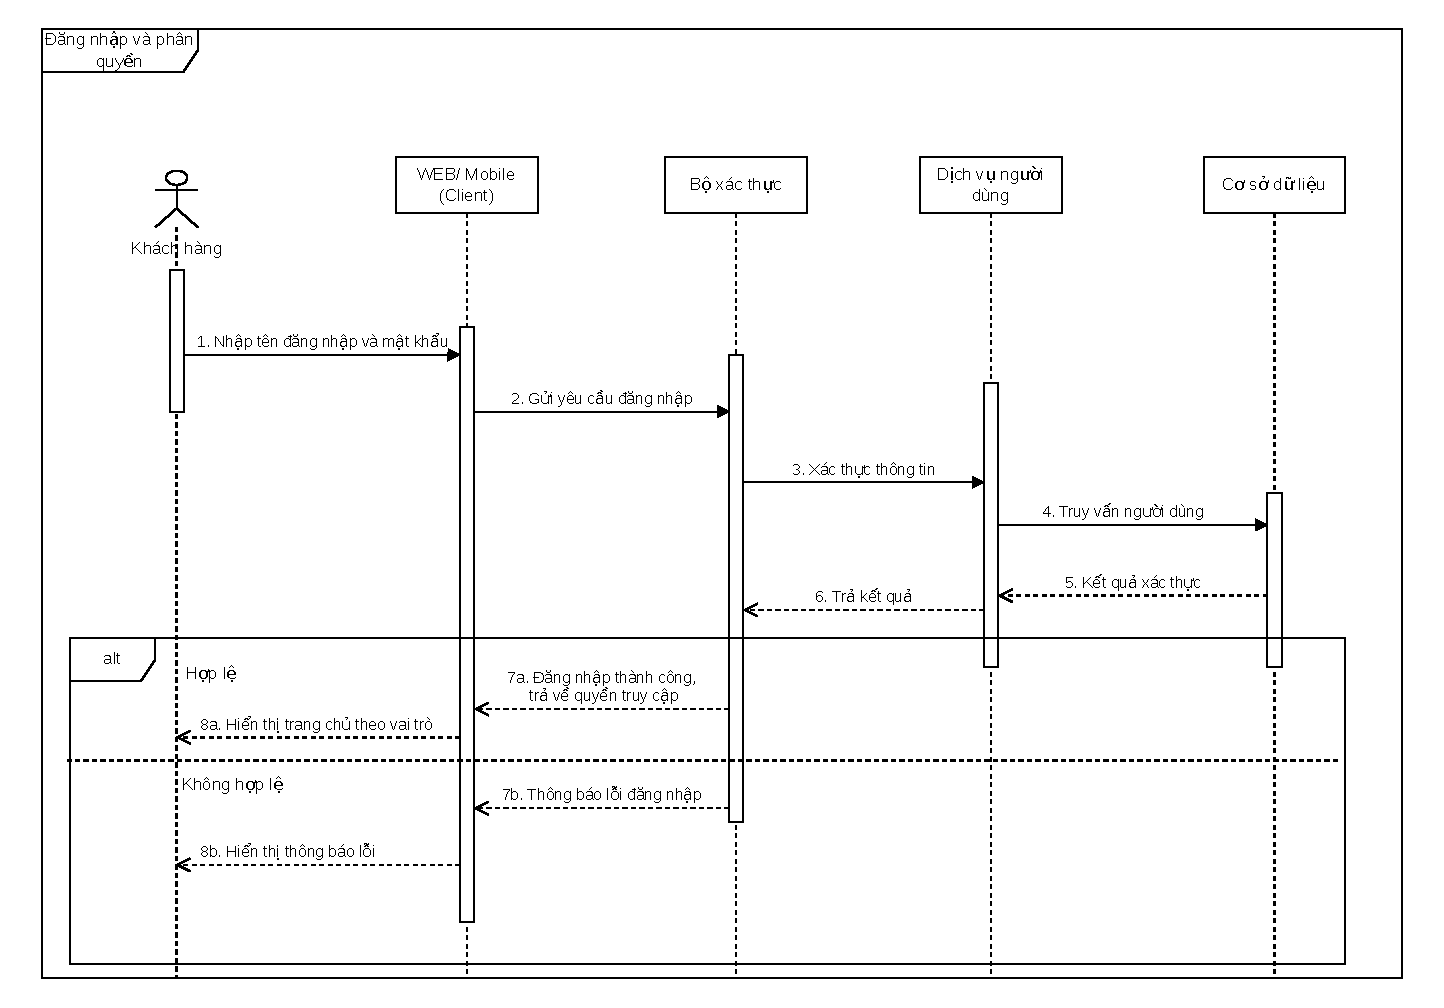
\includegraphics[width=\textwidth]{so-do/sodo-tuantu/Đăng nhập và phân quyền.drawio.pdf}
  \caption{Sơ đồ tuần tự chức năng Đăng nhập và phân quyền}
  \label{fig:seq-uc01}
\end{figure}

\subsection{Tạo Đơn Giao Hàng Mới}

\subsubsection{Sơ Đồ Lớp}
\begin{figure}[H]
  \centering
  
\includegraphics[width=0.85\textwidth]{diagrams/sodolop/UC02_TaoDonHang.png}
  \caption{Sơ đồ lớp chức năng Tạo đơn giao hàng mới}
  \label{fig:class-uc02}
\end{figure}

\subsubsection{Đặc Tả Các Lớp}
\begin{table}[H]
  \centering
  \small
  \begin{tabularx}{\textwidth}{|c|>{\raggedright\arraybackslash}p{3.5cm}|>{\raggedright\arraybackslash}p{4.5cm}|>{\raggedright\arraybackslash}X|}
    \hline
    \textbf{STT} & \textbf{Tên lớp} & \textbf{Thuộc tính / Phương thức} & \textbf{Mô tả} \\
    \hline
    1 & \texttt{Dieu\allowbreak Khien\allowbreak Don\allowbreak Hang} & \texttt{tao\allowbreak Don\allowbreak Hang\allowbreak (yeu\allowbreak Cau)} & REST API controller tiếp nhận yêu cầu tạo đơn giao hàng mới. \\ \hline
    2 & \texttt{Dich\allowbreak Vu\allowbreak Don\allowbreak Hang} & \texttt{tao\allowbreak Don\allowbreak Hang\allowbreak (ma\allowbreak Kh,\allowbreak yeu\allowbreak Cau)}, \texttt{- kiem\allowbreak Tra\allowbreak Tai\allowbreak Trong\allowbreak (can\allowbreak Nang)} & Lớp dịch vụ xử lý logic tạo đơn hàng và kiểm tra giới hạn tải trọng (5kg). \\ \hline
    3 & \texttt{Kho\allowbreak Du\allowbreak Lieu\allowbreak Don\allowbreak Hang} & \texttt{luu\allowbreak (don\allowbreak Hang)} & Interface Repository lưu thông tin đơn hàng mới vào CSDL. \\ \hline
    4 & \texttt{Kho\allowbreak Du\allowbreak Lieu\allowbreak Dia\allowbreak Chi} & \texttt{tim\allowbreak Theo\allowbreak Ma\allowbreak (ma)} & Interface Repository truy vấn thông tin địa chỉ giao hàng của khách. \\ \hline
    5 & \texttt{Yeu\allowbreak Cau\allowbreak Tao\allowbreak Don} & \texttt{ma\allowbreak Dia\allowbreak Chi}, \texttt{loai\allowbreak Hang\allowbreak Hoa}, \texttt{can\allowbreak Nang}, \texttt{kich\allowbreak Co} & DTO đóng gói dữ liệu tạo đơn hàng của khách hàng gửi lên. \\ \hline
    6 & \texttt{Phan\allowbreak Hoi\allowbreak Don\allowbreak Hang} & \texttt{ma\allowbreak Don\allowbreak Hang}, \texttt{trang\allowbreak Thai}, \texttt{ngay\allowbreak Dat\allowbreak Hang} & DTO trả về thông tin cơ bản của đơn hàng sau khi tạo thành công. \\ \hline
    7 & \texttt{Don\allowbreak Hang} & \texttt{ma\allowbreak Don\allowbreak Hang}, \texttt{trang\allowbreak Thai}, \texttt{tong\allowbreak Tien} & Thực thể biểu diễn thông tin đơn giao hàng. \\ \hline
    8 & \texttt{Goi\allowbreak Hang} & \texttt{ma\allowbreak Goi\allowbreak Hang}, \texttt{can\allowbreak Nang} & Thực thể biểu diễn gói hàng đính kèm với đơn hàng. \\ \hline
    9 & \texttt{Dia\allowbreak Chi} & \texttt{ma\allowbreak Dia\allowbreak Chi}, \texttt{dia\allowbreak Chi\allowbreak Cu\allowbreak The} & Thực thể lưu thông tin địa chỉ của khách hàng. \\
    \hline
  \end{tabularx}
  \caption{Đặc tả các lớp chức năng Tạo Đơn Giao Hàng Mới}
  \label{tab:class-spec-uc02}
\end{table}

\subsubsection{Sơ Đồ Tuần Tự}
\begin{figure}[H]
  \centering
  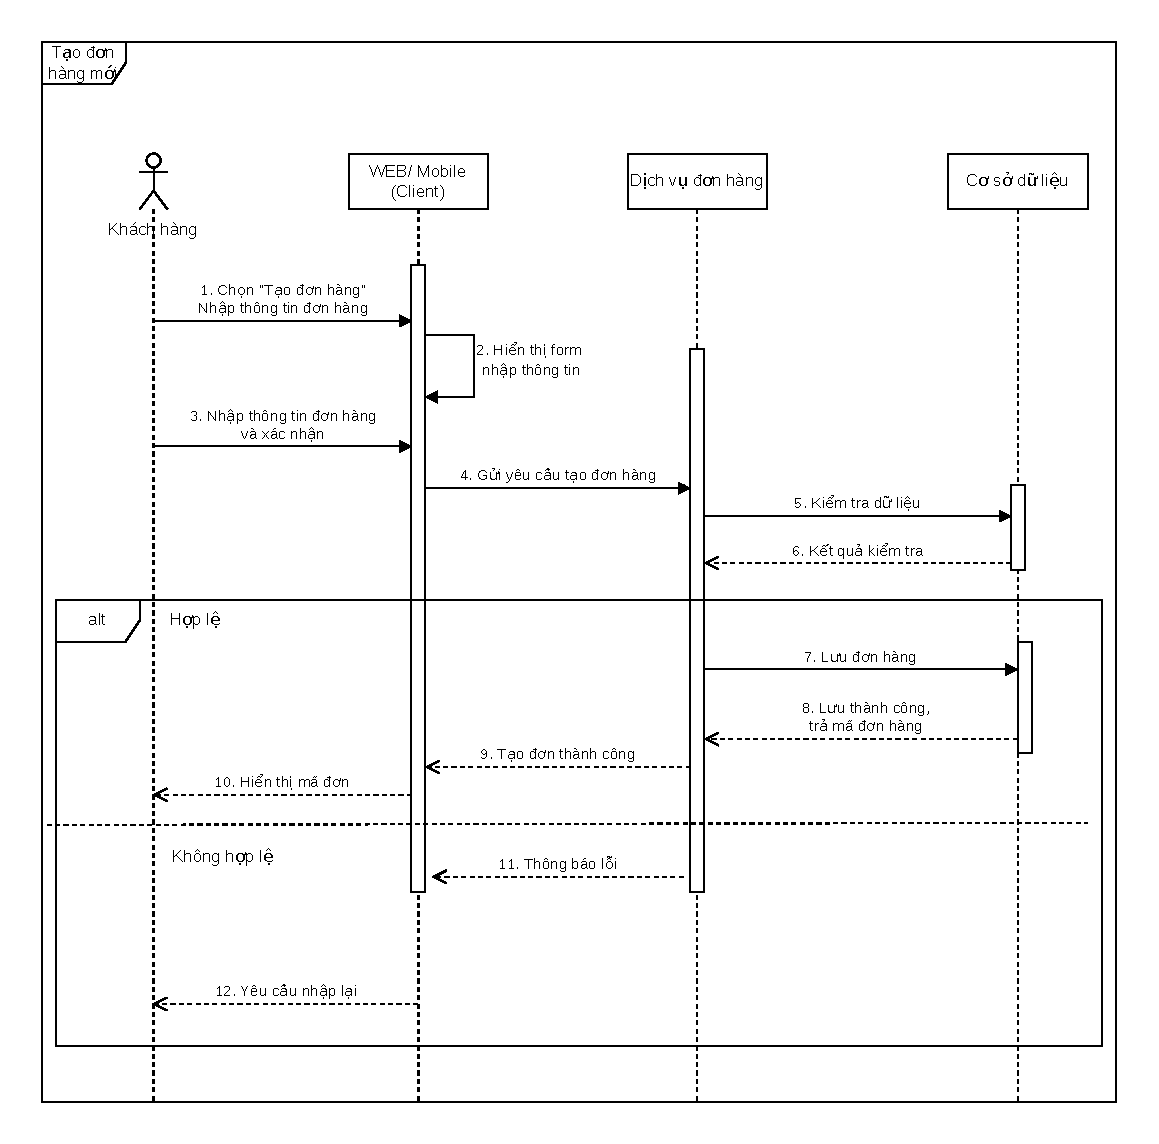
\includegraphics[width=\textwidth]{so-do/sodo-tuantu/Tạo đơn hàng mới.drawio.pdf}
  \caption{Sơ đồ tuần tự chức năng Tạo đơn hàng mới}
  \label{fig:seq-uc02}
\end{figure}

\subsection{Cập Nhật và Hủy Đơn Giao Hàng}

\subsubsection{Sơ Đồ Lớp}
\begin{figure}[H]
  \centering
  
\includegraphics[width=0.8\textwidth]{diagrams/sodolop/UC03_CapNhatHuyDon.png}
  \caption{Sơ đồ lớp chức năng Cập nhật và Hủy đơn giao hàng}
  \label{fig:class-uc03}
\end{figure}

\subsubsection{Đặc Tả Các Lớp}
\begin{table}[H]
  \centering
  \small
  \begin{tabularx}{\textwidth}{|c|>{\raggedright\arraybackslash}p{3.5cm}|>{\raggedright\arraybackslash}p{4.5cm}|>{\raggedright\arraybackslash}X|}
    \hline
    \textbf{STT} & \textbf{Tên lớp} & \textbf{Thuộc tính / Phương thức} & \textbf{Mô tả} \\
    \hline
    1 & \texttt{Dieu\allowbreak Khien\allowbreak Don\allowbreak Hang} & \texttt{cap\allowbreak Nhat\allowbreak Don\allowbreak Hang\allowbreak (ma,\allowbreak yeu\allowbreak Cau)}, \texttt{huy\allowbreak Don\allowbreak Hang\allowbreak (ma)} & REST API controller tiếp nhận yêu cầu sửa/hủy đơn hàng. \\ \hline
    2 & \texttt{Dich\allowbreak Vu\allowbreak Don\allowbreak Hang} & \texttt{cap\allowbreak Nhat\allowbreak Don\allowbreak Hang\allowbreak (...)},\newline \texttt{huy\allowbreak Don\allowbreak Hang\allowbreak (...)},\newline \texttt{- kiem\allowbreak Tra\allowbreak Trang\allowbreak Thai\allowbreak Cho\allowbreak Phep\allowbreak Sua\allowbreak (tt)} & Dịch vụ xử lý nghiệp vụ cập nhật/hủy đơn và kiểm tra điều kiện trạng thái "Chờ duyệt". \\ \hline
    3 & \texttt{Kho\allowbreak Du\allowbreak Lieu\allowbreak Don\allowbreak Hang} & \texttt{tim\allowbreak Theo\allowbreak Ma\allowbreak (ma)}, \texttt{luu\allowbreak (don\allowbreak Hang)} & Interface Repository tìm kiếm và lưu thông tin cập nhật đơn hàng. \\ \hline
    4 & \texttt{Yeu\allowbreak Cau\allowbreak Cap\allowbreak Nhat\allowbreak Don} & \texttt{ma\allowbreak Dia\allowbreak Chi}, \texttt{ghi\allowbreak Chu} & DTO đóng gói các thông tin muốn thay đổi của đơn hàng. \\ \hline
    5 & \texttt{Phan\allowbreak Hoi\allowbreak Don\allowbreak Hang} & \texttt{ma\allowbreak Don\allowbreak Hang}, \texttt{trang\allowbreak Thai} & DTO trả về kết quả trạng thái mới của đơn hàng sau chỉnh sửa. \\ \hline
    6 & \texttt{Don\allowbreak Hang} & \texttt{ma\allowbreak Don\allowbreak Hang}, \texttt{trang\allowbreak Thai}, \texttt{huy\allowbreak Don\allowbreak Hang\allowbreak ()} & Thực thể đơn hàng chứa phương thức đổi trạng thái sang "Đã hủy". \\
    \hline
  \end{tabularx}
  \caption{Đặc tả các lớp chức năng Cập Nhật và Hủy Đơn Giao Hàng}
  \label{tab:class-spec-uc03}
\end{table}

\subsubsection{Sơ Đồ Tuần Tự}
\begin{figure}[H]
  \centering
  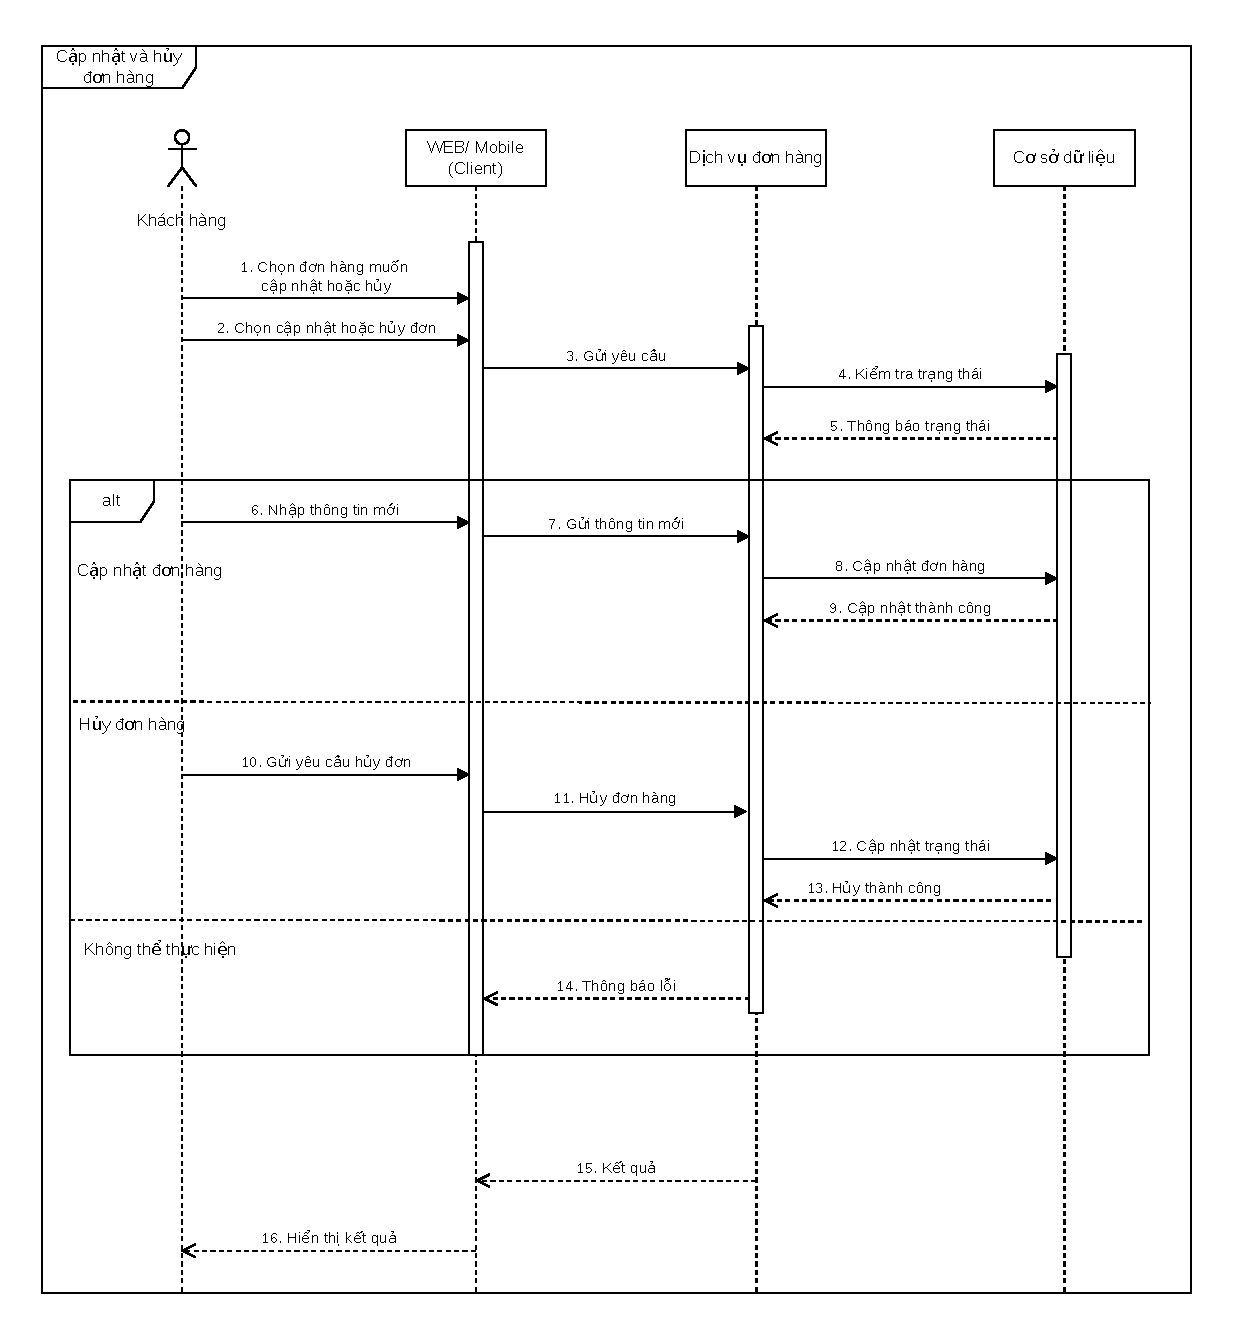
\includegraphics[width=\textwidth]{so-do/sodo-tuantu/Cập nhật và hủy đơn hàng.drawio.pdf}
  \caption{Sơ đồ tuần tự chức năng Cập nhật và hủy đơn hàng}
  \label{fig:seq-uc03}
\end{figure}

\subsection{Phê Duyệt Yêu Cầu Giao Hàng}

\subsubsection{Sơ Đồ Lớp}
\begin{figure}[H]
  \centering
  
\includegraphics[width=0.85\textwidth]{diagrams/sodolop/UC04_PheDuyetYeuCau.png}
  \caption{Sơ đồ lớp chức năng Phê duyệt yêu cầu giao hàng}
  \label{fig:class-uc04}
\end{figure}

\subsubsection{Đặc Tả Các Lớp}
\begin{table}[H]
  \centering
  \small
  \begin{tabularx}{\textwidth}{|c|>{\raggedright\arraybackslash}p{3.5cm}|>{\raggedright\arraybackslash}p{4.5cm}|>{\raggedright\arraybackslash}X|}
    \hline
    \textbf{STT} & \textbf{Tên lớp} & \textbf{Thuộc tính / Phương thức} & \textbf{Mô tả} \\
    \hline
    1 & \texttt{Dieu\allowbreak Khien\allowbreak Phe\allowbreak Duyet} & \texttt{duyet\allowbreak Don\allowbreak (ma)}, \texttt{tu\allowbreak Choi\allowbreak Don\allowbreak (ma,\allowbreak yeu\allowbreak Cau)} & REST API controller tiếp nhận quyết định duyệt/từ chối từ điều phối viên. \\ \hline
    2 & \texttt{Dich\allowbreak Vu\allowbreak Dieu\allowbreak Phoi} & \texttt{duyet\allowbreak Don\allowbreak (ma)}, \texttt{tu\allowbreak Choi\allowbreak Don\allowbreak (ma,\allowbreak ly\allowbreak Do)}, \texttt{- kiem\allowbreak Tra\allowbreak Tram\allowbreak Kha\allowbreak Dung\allowbreak (ma\allowbreak Dia\allowbreak Chi)} & Dịch vụ xử lý phê duyệt đơn và kiểm tra sự tồn tại của trạm drone khả dụng gần đó. \\ \hline
    3 & \texttt{Kho\allowbreak Du\allowbreak Lieu\allowbreak Don\allowbreak Hang} & \texttt{tim\allowbreak Theo\allowbreak Ma\allowbreak (ma)}, \texttt{luu\allowbreak (don\allowbreak Hang)} & Interface Repository cập nhật trạng thái đã duyệt/bị từ chối của đơn hàng. \\ \hline
    4 & \texttt{Kho\allowbreak Du\allowbreak Lieu\allowbreak Tram\allowbreak Ha\allowbreak Canh} & \texttt{tim\allowbreak Gan\allowbreak Nhat\allowbreak (lat,\allowbreak lng)} & Interface Repository tìm trạm hạ cánh gần vị trí giao để kiểm tra khả dụng. \\ \hline
    5 & \texttt{Yeu\allowbreak Cau\allowbreak Tu\allowbreak Choi} & \texttt{ly\allowbreak Do} & DTO chứa lý do từ chối phê duyệt đơn hàng. \\ \hline
    6 & \texttt{Phan\allowbreak Hoi\allowbreak Don\allowbreak Hang} & \texttt{ma\allowbreak Don\allowbreak Hang}, \texttt{trang\allowbreak Thai} & DTO phản hồi kết quả duyệt hoặc từ chối đơn hàng. \\ \hline
    7 & \texttt{Don\allowbreak Hang} & \texttt{ma\allowbreak Don\allowbreak Hang}, \texttt{trang\allowbreak Thai} & Thực thể đơn hàng lưu trạng thái hiện tại. \\ \hline
    8 & \texttt{Tram\allowbreak Ha\allowbreak Canh} & \texttt{ma\allowbreak Tram}, \texttt{trang\allowbreak Thai\allowbreak Hoat\allowbreak Dong} & Thực thể trạm hạ cánh kiểm tra trạm có đang hoạt động tốt hay không. \\
    \hline
  \end{tabularx}
  \caption{Đặc tả các lớp chức năng Phê Duyệt Yêu Cầu Giao Hàng}
  \label{tab:class-spec-uc04}
\end{table}

\subsection{Lập Lịch Giao Hàng}

\subsubsection{Sơ Đồ Lớp}
\begin{figure}[H]
  \centering
  
\includegraphics[width=0.85\textwidth]{diagrams/sodolop/UC05_LapLichGiao.png}
  \caption{Sơ đồ lớp chức năng Lập lịch giao hàng}
  \label{fig:class-uc05}
\end{figure}

\subsubsection{Đặc Tả Các Lớp}
\begin{table}[H]
  \centering
  \small
  \begin{tabularx}{\textwidth}{|c|>{\raggedright\arraybackslash}p{3.5cm}|>{\raggedright\arraybackslash}p{4.5cm}|>{\raggedright\arraybackslash}X|}
    \hline
    \textbf{STT} & \textbf{Tên lớp} & \textbf{Thuộc tính / Phương thức} & \textbf{Mô tả} \\
    \hline
    1 & \texttt{Dieu\allowbreak Khien\allowbreak Lap\allowbreak Lich} & \texttt{lap\allowbreak Lich\allowbreak Giao\allowbreak Hang\allowbreak (ma\allowbreak Don\allowbreak Hang,\allowbreak yeu\allowbreak Cau)} & REST API controller tiếp nhận yêu cầu lập lịch chuyến bay. \\ \hline
    2 & \texttt{Dich\allowbreak Vu\allowbreak Lap\allowbreak Lich} & \texttt{lap\allowbreak Lich\allowbreak Giao\allowbreak (ma\allowbreak Don\allowbreak Hang,\allowbreak yeu\allowbreak Cau)},\newline \texttt{- tim\allowbreak Tram\allowbreak Kha\allowbreak Dung\allowbreak (ma\allowbreak Dia\allowbreak Chi)} & Dịch vụ lập lịch, kiểm tra điều kiện của trạm và khởi tạo thông tin chuyến đi. \\ \hline
    3 & \texttt{Kho\allowbreak Du\allowbreak Lieu\allowbreak Tram\allowbreak Ha\allowbreak Canh} & \texttt{tim\allowbreak Tat\allowbreak Ca\allowbreak ()}, \texttt{tim\allowbreak Theo\allowbreak Ma\allowbreak (ma)} & Interface Repository kiểm tra cấu hình trạm trong CSDL. \\ \hline
    4 & \texttt{Kho\allowbreak Du\allowbreak Lieu\allowbreak Giao\allowbreak Hang} & \texttt{luu\allowbreak (giao\allowbreak Hang)} & Interface Repository lưu trữ thông tin chuyến giao hàng mới lên lịch. \\ \hline
    5 & \texttt{Yeu\allowbreak Cau\allowbreak Lap\allowbreak Lich} & \texttt{ma\allowbreak Tram}, \texttt{thoi\allowbreak Gian\allowbreak Du\allowbreak Kien} & DTO chứa mã trạm hạ cánh và mốc thời gian giao hàng dự kiến. \\ \hline
    6 & \texttt{Phan\allowbreak Hoi\allowbreak Giao\allowbreak Hang} & \texttt{ma\allowbreak Giao\allowbreak Hang}, \texttt{trang\allowbreak Thai}, \texttt{ma\allowbreak Tram} & DTO phản hồi kết quả thiết lập lịch trình chuyến đi của drone. \\ \hline
    7 & \texttt{Giao\allowbreak Hang} & \texttt{ma\allowbreak Giao\allowbreak Hang}, \texttt{trang\allowbreak Thai} & Thực thể biểu diễn chuyến đi giao hàng bằng drone. \\ \hline
    8 & \texttt{Tram\allowbreak Ha\allowbreak Canh} & \texttt{ma\allowbreak Tram}, \texttt{cong\allowbreak Suat\allowbreak Toi\allowbreak Da}, \texttt{kiem\allowbreak Tra\allowbreak Suc\allowbreak Chua\allowbreak ()} & Thực thể trạm hạ cánh kiểm tra sức chứa hiện tại có bị quá tải. \\ \hline
    9 & \texttt{Don\allowbreak Hang} & \texttt{ma\allowbreak Don\allowbreak Hang} & Thực thể đơn hàng được gắn lịch giao. \\
    \hline
  \end{tabularx}
  \caption{Đặc tả các lớp chức năng Lập Lịch Giao Hàng}
  \label{tab:class-spec-uc05}
\end{table}

\subsection{Xử Lý Giao Hàng Thất Bại}

\subsubsection{Sơ Đồ Lớp}
\begin{figure}[H]
  \centering
  
\includegraphics[width=0.85\textwidth]{diagrams/sodolop/UC06_XuLyGiaoThatBai.png}
  \caption{Sơ đồ lớp chức năng Xử lý giao hàng thất bại}
  \label{fig:class-uc06}
\end{figure}

\subsubsection{Đặc Tả Các Lớp}
\begin{table}[H]
  \centering
  \small
  \begin{tabularx}{\textwidth}{|c|>{\raggedright\arraybackslash}p{3.5cm}|>{\raggedright\arraybackslash}p{4.5cm}|>{\raggedright\arraybackslash}X|}
    \hline
    \textbf{STT} & \textbf{Tên lớp} & \textbf{Thuộc tính / Phương thức} & \textbf{Mô tả} \\
    \hline
    1 & \texttt{Dieu\allowbreak Khien\allowbreak Giao\allowbreak Hang} & \texttt{xu\allowbreak Ly\allowbreak Giao\allowbreak That\allowbreak Bai\allowbreak (ma,\allowbreak yeu\allowbreak Cau)},\newline \texttt{giao\allowbreak Lai\allowbreak (ma)} & REST API controller tiếp nhận thông báo sự cố giao hàng thất bại. \\ \hline
    2 & \texttt{Dich\allowbreak Vu\allowbreak Giao\allowbreak Hang} & \texttt{xu\allowbreak Ly\allowbreak Giao\allowbreak That\allowbreak Bai\allowbreak (...)},\newline \texttt{giao\allowbreak Lai\allowbreak (...)} & Dịch vụ xử lý nghiệp vụ ghi nhận sự cố của chuyến bay và yêu cầu drone quay đầu hoặc giao lại. \\ \hline
    3 & \texttt{Kho\allowbreak Du\allowbreak Lieu\allowbreak Giao\allowbreak Hang} & \texttt{tim\allowbreak Theo\allowbreak Ma\allowbreak (ma)}, \texttt{luu\allowbreak (giao\allowbreak Hang)} & Interface Repository cập nhật trạng thái chuyến giao hàng thành giao thất bại. \\ \hline
    4 & \texttt{Kho\allowbreak Du\allowbreak Lieu\allowbreak Su\allowbreak Co} & \texttt{luu\allowbreak (su\allowbreak Co)} & Interface Repository lưu vết vụ việc sự cố phát sinh của drone. \\ \hline
    5 & \texttt{Yeu\allowbreak Cau\allowbreak Su\allowbreak Co} & \texttt{ly\allowbreak Do}, \texttt{muc\allowbreak Do\allowbreak Nghiem\allowbreak Trong} & DTO chứa chi tiết báo cáo sự cố (do thời tiết, hỏng pin, v.v.). \\ \hline
    6 & \texttt{Phan\allowbreak Hoi\allowbreak Giao\allowbreak Hang} & \texttt{ma\allowbreak Giao\allowbreak Hang}, \texttt{trang\allowbreak Thai} & DTO trả về trạng thái mới của chuyến giao hàng sau khi xử lý sự cố. \\ \hline
    7 & \texttt{Giao\allowbreak Hang} & \texttt{ma\allowbreak Giao\allowbreak Hang}, \texttt{trang\allowbreak Thai} & Thực thể chuyến giao hàng liên kết với các sự cố xảy ra. \\ \hline
    8 & \texttt{Su\allowbreak Co\allowbreak Giao\allowbreak Hang} & \texttt{ma\allowbreak Van\allowbreak De}, \texttt{mo\allowbreak Ta\allowbreak Su\allowbreak Co}, \texttt{muc\allowbreak Do\allowbreak Nghiem\allowbreak Trong} & Thực thể lưu thông tin chi tiết sự cố phục vụ thống kê phân tích. \\
    \hline
  \end{tabularx}
  \caption{Đặc tả các lớp chức năng Xử Lý Giao Hàng Thất Bại}
  \label{tab:class-spec-uc06}
\end{table}

\subsection{Xác Nhận Nhận/Gửi Kiện Hàng Tại Trạm}

\subsubsection{Sơ Đồ Lớp}
\begin{figure}[H]
  \centering
  
\includegraphics[width=0.85\textwidth]{diagrams/sodolop/UC07_XacNhanKienHangTaiTram.png}
  \caption{Sơ đồ lớp chức năng Xác nhận nhận/gửi kiện hàng tại trạm}
  \label{fig:class-uc07}
\end{figure}

\subsubsection{Đặc Tả Các Lớp}
\begin{table}[H]
  \centering
  \small
  \begin{tabularx}{\textwidth}{|c|>{\raggedright\arraybackslash}p{3.5cm}|>{\raggedright\arraybackslash}p{4.5cm}|>{\raggedright\arraybackslash}X|}
    \hline
    \textbf{STT} & \textbf{Tên lớp} & \textbf{Thuộc tính / Phương thức} & \textbf{Mô tả} \\
    \hline
    1 & \texttt{Dieu\allowbreak Khien\allowbreak Tram} & \texttt{xac\allowbreak Nhan\allowbreak Nhan\allowbreak Kien\allowbreak Hang\allowbreak (ma\allowbreak Don\allowbreak Hang)},\newline \texttt{xac\allowbreak Nhan\allowbreak Xuat\allowbreak Ben\allowbreak (ma\allowbreak Giao\allowbreak Hang)} & REST API controller tiếp nhận cập nhật kiểm kho tại trạm. \\ \hline
    2 & \texttt{Dich\allowbreak Vu\allowbreak Kien\allowbreak Hang} & \texttt{kiem\allowbreak Tra\allowbreak Kien\allowbreak Hang\allowbreak (ma\allowbreak Don\allowbreak Hang)},\newline \texttt{cap\allowbreak Nhat\allowbreak Trang\allowbreak Thai\allowbreak Kien\allowbreak Hang\allowbreak (...)} & Dịch vụ xử lý quét mã vạch nhận kiện hàng vào trạm lưu kho tạm thời. \\ \hline
    3 & \texttt{Dich\allowbreak Vu\allowbreak Giao\allowbreak Hang} & \texttt{cap\allowbreak Nhat\allowbreak Trang\allowbreak Thai\allowbreak Giao\allowbreak (ma,\allowbreak tt)} & Dịch vụ kích hoạt trạng thái "Đang giao" khi drone cất cánh rời trạm. \\ \hline
    4 & \texttt{Kho\allowbreak Du\allowbreak Lieu\allowbreak Goi\allowbreak Hang} & \texttt{tim\allowbreak Theo\allowbreak Ma\allowbreak Don\allowbreak Hang\allowbreak (ma)}, \texttt{luu\allowbreak (goi\allowbreak Hang)} & Interface Repository quản lý trạng thái hiện thời của kiện hàng. \\ \hline
    5 & \texttt{Kho\allowbreak Du\allowbreak Lieu\allowbreak Giao\allowbreak Hang} & \texttt{luu\allowbreak (giao\allowbreak Hang)} & Interface Repository lưu trữ sự kiện drone xuất bến. \\ \hline
    6 & \texttt{Phan\allowbreak Hoi\allowbreak Kien\allowbreak Hang} & \texttt{ma\allowbreak Goi\allowbreak Hang}, \texttt{trang\allowbreak Thai} & DTO phản hồi trạng thái gói hàng khi đã nhập kho trạm thành công. \\ \hline
    7 & \texttt{Phan\allowbreak Hoi\allowbreak Giao\allowbreak Hang} & \texttt{ma\allowbreak Giao\allowbreak Hang}, \texttt{trang\allowbreak Thai} & DTO phản hồi trạng thái xuất phát của drone. \\ \hline
    8 & \texttt{Goi\allowbreak Hang} & \texttt{ma\allowbreak Goi\allowbreak Hang}, \texttt{can\allowbreak Nang} & Thực thể kiện hàng lưu kho tại trạm hạ cánh. \\ \hline
    9 & \texttt{Giao\allowbreak Hang} & \texttt{ma\allowbreak Giao\allowbreak Hang}, \texttt{trang\allowbreak Thai} & Thực thể chuyến bay của drone. \\
    \hline
  \end{tabularx}
  \caption{Đặc tả các lớp chức năng Xác Nhận Nhận/Gửi Kiện Hàng Tại Trạm}
  \label{tab:class-spec-uc07}
\end{table}

\subsubsection{Sơ Đồ Tuần Tự}
\begin{figure}[H]
  \centering
  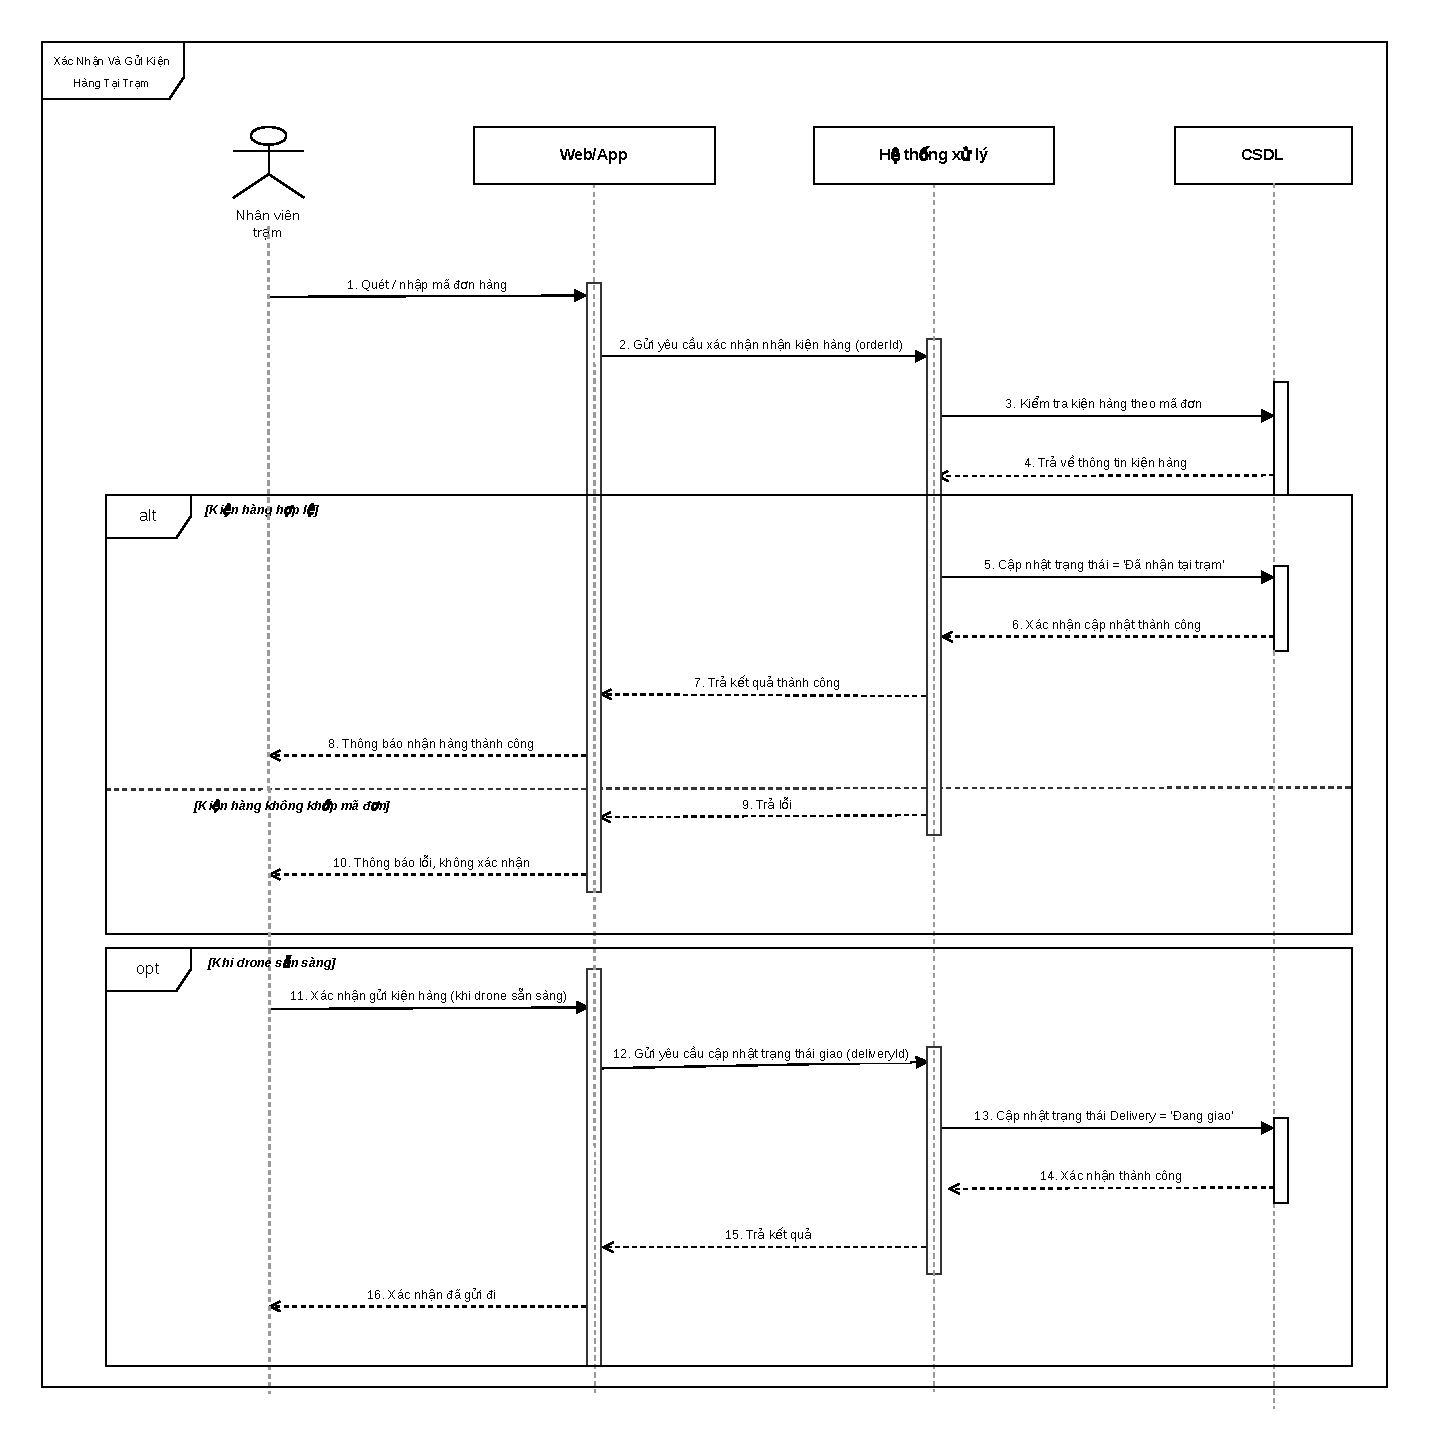
\includegraphics[width=\textwidth]{so-do/sodo-tuantu/Xác Nhận Nhận_Gửi Kiện Hàng Tại Trạm.drawio.pdf}
  \caption{Sơ đồ tuần tự chức năng Xác nhận nhận và gửi kiện hàng tại trạm}
  \label{fig:seq-uc07}
\end{figure}

\subsection{Theo Dõi Giao Hàng Thời Gian Thực}

\subsubsection{Sơ Đồ Lớp}
\begin{figure}[H]
  \centering
  
\includegraphics[width=0.85\textwidth]{diagrams/sodolop/UC08_TheoDoiGiaoHangRealtime.png}
  \caption{Sơ đồ lớp chức năng Theo dõi giao hàng thời gian thực}
  \label{fig:class-uc08}
\end{figure}

\subsubsection{Đặc Tả Các Lớp}
\begin{table}[H]
  \centering
  \small
  \begin{tabularx}{\textwidth}{|c|>{\raggedright\arraybackslash}p{3.5cm}|>{\raggedright\arraybackslash}p{4.5cm}|>{\raggedright\arraybackslash}X|}
    \hline
    \textbf{STT} & \textbf{Tên lớp} & \textbf{Thuộc tính / Phương thức} & \textbf{Mô tả} \\
    \hline
    1 & \texttt{Dieu\allowbreak Khien\allowbreak Theo\allowbreak Doi} & \texttt{lay\allowbreak Thong\allowbreak Tin\allowbreak Theo\allowbreak Doi\allowbreak (ma\allowbreak Giao\allowbreak Hang)} & REST API controller phục vụ truy vấn thông tin hành trình. \\ \hline
    2 & \texttt{Dich\allowbreak Vu\allowbreak Theo\allowbreak Doi} & \texttt{lay\allowbreak Vi\allowbreak Tri\allowbreak Hien\allowbreak Tai\allowbreak (ma\allowbreak Giao\allowbreak Hang)},\newline \texttt{dang\allowbreak Ky\allowbreak Kenh\allowbreak Truc\allowbreak Tuyen\allowbreak (ma\allowbreak Giao\allowbreak Hang)},\newline \texttt{huy\allowbreak Dang\allowbreak Ky\allowbreak Kenh\allowbreak Truc\allowbreak Tuyen\allowbreak (ma\allowbreak Giao\allowbreak Hang)} & Dịch vụ xử lý đăng ký kênh truyền và đồng bộ dữ liệu vị trí GPS thực tế. \\ \hline
    3 & \texttt{Kho\allowbreak Du\allowbreak Lieu\allowbreak Giao\allowbreak Hang} & \texttt{tim\allowbreak Theo\allowbreak Ma\allowbreak (ma)} & Interface Repository truy vấn tọa độ GPS hiện tại của chuyến giao hàng. \\ \hline
    4 & \texttt{Kenh\allowbreak Truc\allowbreak Tuyen\allowbreak Thoi\allowbreak Gian\allowbreak Thuc} & \texttt{dang\allowbreak Ky\allowbreak Kenh\allowbreak (ten\allowbreak Kenh)},\newline \texttt{huy\allowbreak Dang\allowbreak Ky\allowbreak Kenh\allowbreak (ten\allowbreak Kenh)},\newline \texttt{khi\allowbreak Co\allowbreak Cap\allowbreak Nhat\allowbreak (ham\allowbreak Xu\allowbreak Ly)} & Cổng WebSocket hoặc Supabase Realtime channel đẩy vị trí drone liên tục cho client. \\ \hline
    5 & \texttt{Phan\allowbreak Hoi\allowbreak Theo\allowbreak Doi} & \texttt{vi\allowbreak Do}, \texttt{kinh\allowbreak Do}, \texttt{trang\allowbreak Thai}, \texttt{thoi\allowbreak Gian\allowbreak Cap\allowbreak Nhat} & DTO đóng gói tọa độ GPS thời gian thực trả về cho bản đồ phía người dùng. \\ \hline
    6 & \texttt{Giao\allowbreak Hang} & \texttt{ma\allowbreak Giao\allowbreak Hang}, \texttt{vi\allowbreak Tri\allowbreak Hien\allowbreak Tai\allowbreak Lat},\newline \texttt{vi\allowbreak Tri\allowbreak Hien\allowbreak Tai\allowbreak Lng}, \texttt{cap\allowbreak Nhat\allowbreak Vi\allowbreak Tri\allowbreak (lat,\allowbreak lng)} & Thực thể chuyến giao hàng lưu thông tin tọa độ động của thiết bị drone. \\
    \hline
  \end{tabularx}
  \caption{Đặc tả các lớp chức năng Theo Dõi Giao Hàng Thời Gian Thực}
  \label{tab:class-spec-uc08}
\end{table}

\subsubsection{Sơ Đồ Tuần Tự}
\begin{figure}[H]
  \centering
  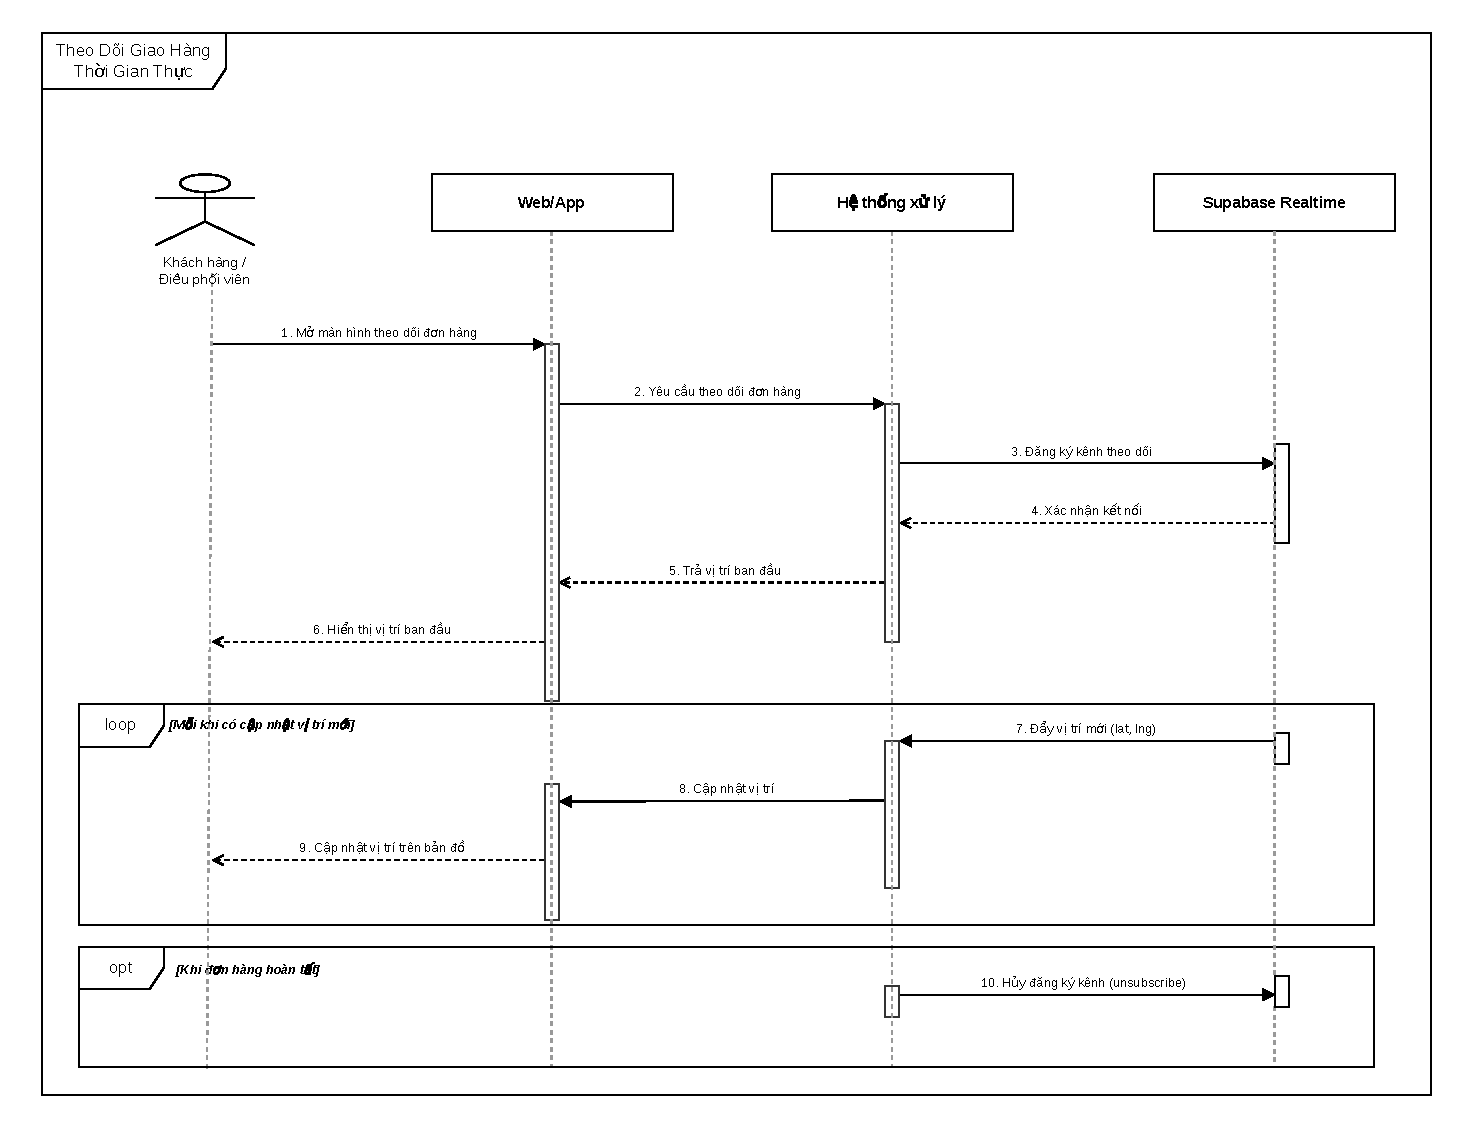
\includegraphics[width=\textwidth]{so-do/sodo-tuantu/Theo Dõi Giao Hàng Thời Gian Thực.drawio.pdf}
  \caption{Sơ đồ tuần tự chức năng Theo dõi giao hàng thời gian thực}
  \label{fig:seq-uc08}
\end{figure}

\subsection{Xác Nhận Giao Hàng Thành Công}

\subsubsection{Sơ Đồ Lớp}
\begin{figure}[H]
  \centering
  
\includegraphics[width=0.85\textwidth]{diagrams/sodolop/UC09_XacNhanGiaoThanhCong.png}
  \caption{Sơ đồ lớp chức năng Xác nhận giao hàng thành công}
  \label{fig:class-uc09}
\end{figure}

\subsubsection{Đặc Tả Các Lớp}
\begin{table}[H]
  \centering
  \small
  \begin{tabularx}{\textwidth}{|c|>{\raggedright\arraybackslash}p{3.5cm}|>{\raggedright\arraybackslash}p{4.5cm}|>{\raggedright\arraybackslash}X|}
    \hline
    \textbf{STT} & \textbf{Tên lớp} & \textbf{Thuộc tính / Phương thức} & \textbf{Mô tả} \\
    \hline
    1 & \texttt{Dieu\allowbreak Khien\allowbreak Giao\allowbreak Hang} & \texttt{xac\allowbreak Nhan\allowbreak Giao\allowbreak Thanh\allowbreak Cong\allowbreak (ma\allowbreak Giao\allowbreak Hang)} & REST API controller tiếp nhận lệnh xác nhận đã nhận hàng. \\ \hline
    2 & \texttt{Dich\allowbreak Vu\allowbreak Giao\allowbreak Hang} & \texttt{xac\allowbreak Nhan\allowbreak Giao\allowbreak Thanh\allowbreak Cong\allowbreak (ma\allowbreak Giao\allowbreak Hang)} & Dịch vụ thực hiện chuyển đổi trạng thái đơn hàng và drone sang hoàn tất. \\ \hline
    3 & \texttt{Dich\allowbreak Vu\allowbreak Thong\allowbreak Bao} & \texttt{gui\allowbreak Thong\allowbreak Bao\allowbreak (ma\allowbreak Kh,\allowbreak noi\allowbreak Dung)} & Dịch vụ gửi thông báo hoàn tất đơn qua email hoặc đẩy thông báo ứng dụng. \\ \hline
    4 & \texttt{Kho\allowbreak Du\allowbreak Lieu\allowbreak Giao\allowbreak Hang} & \texttt{tim\allowbreak Theo\allowbreak Ma\allowbreak (ma)}, \texttt{luu\allowbreak (giao\allowbreak Hang)} & Interface Repository cập nhật trạng thái chuyến giao hàng thành "Đã giao". \\ \hline
    5 & \texttt{Kho\allowbreak Du\allowbreak Lieu\allowbreak Don\allowbreak Hang} & \texttt{luu\allowbreak (don\allowbreak Hang)} & Interface Repository cập nhật trạng thái đơn thành "Đã giao thành công". \\ \hline
    6 & \texttt{Kho\allowbreak Du\allowbreak Lieu\allowbreak Thong\allowbreak Bao} & \texttt{luu\allowbreak (thong\allowbreak Bao)} & Interface Repository lưu nhật ký thông báo điện tử gửi cho khách. \\ \hline
    7 & \texttt{Phan\allowbreak Hoi\allowbreak Xac\allowbreak Nhan} & \texttt{ma\allowbreak Giao\allowbreak Hang}, \texttt{trang\allowbreak Thai}, \texttt{thoi\allowbreak Gian\allowbreak Giao} & DTO phản hồi xác nhận thành công bao gồm dấu mốc thời gian nhận hàng. \\ \hline
    8 & \texttt{Giao\allowbreak Hang} & \texttt{ma\allowbreak Giao\allowbreak Hang}, \texttt{trang\allowbreak Thai} & Thực thể chuyến đi giao hàng. \\ \hline
    9 & \texttt{Don\allowbreak Hang} & \texttt{ma\allowbreak Don\allowbreak Hang}, \texttt{trang\allowbreak Thai} & Thực thể đơn hàng. \\ \hline
    10 & \texttt{Thong\allowbreak Bao} & \texttt{ma\allowbreak Thong\allowbreak Bao}, \texttt{noi\allowbreak Dung} & Thực thể lưu thông báo gửi cho khách hàng. \\
    \hline
  \end{tabularx}
  \caption{Đặc tả các lớp chức năng Xác Nhận Giao Hàng Thành Công}
  \label{tab:class-spec-uc09}
\end{table}

\subsubsection{Sơ Đồ Tuần Tự}
\begin{figure}[H]
  \centering
  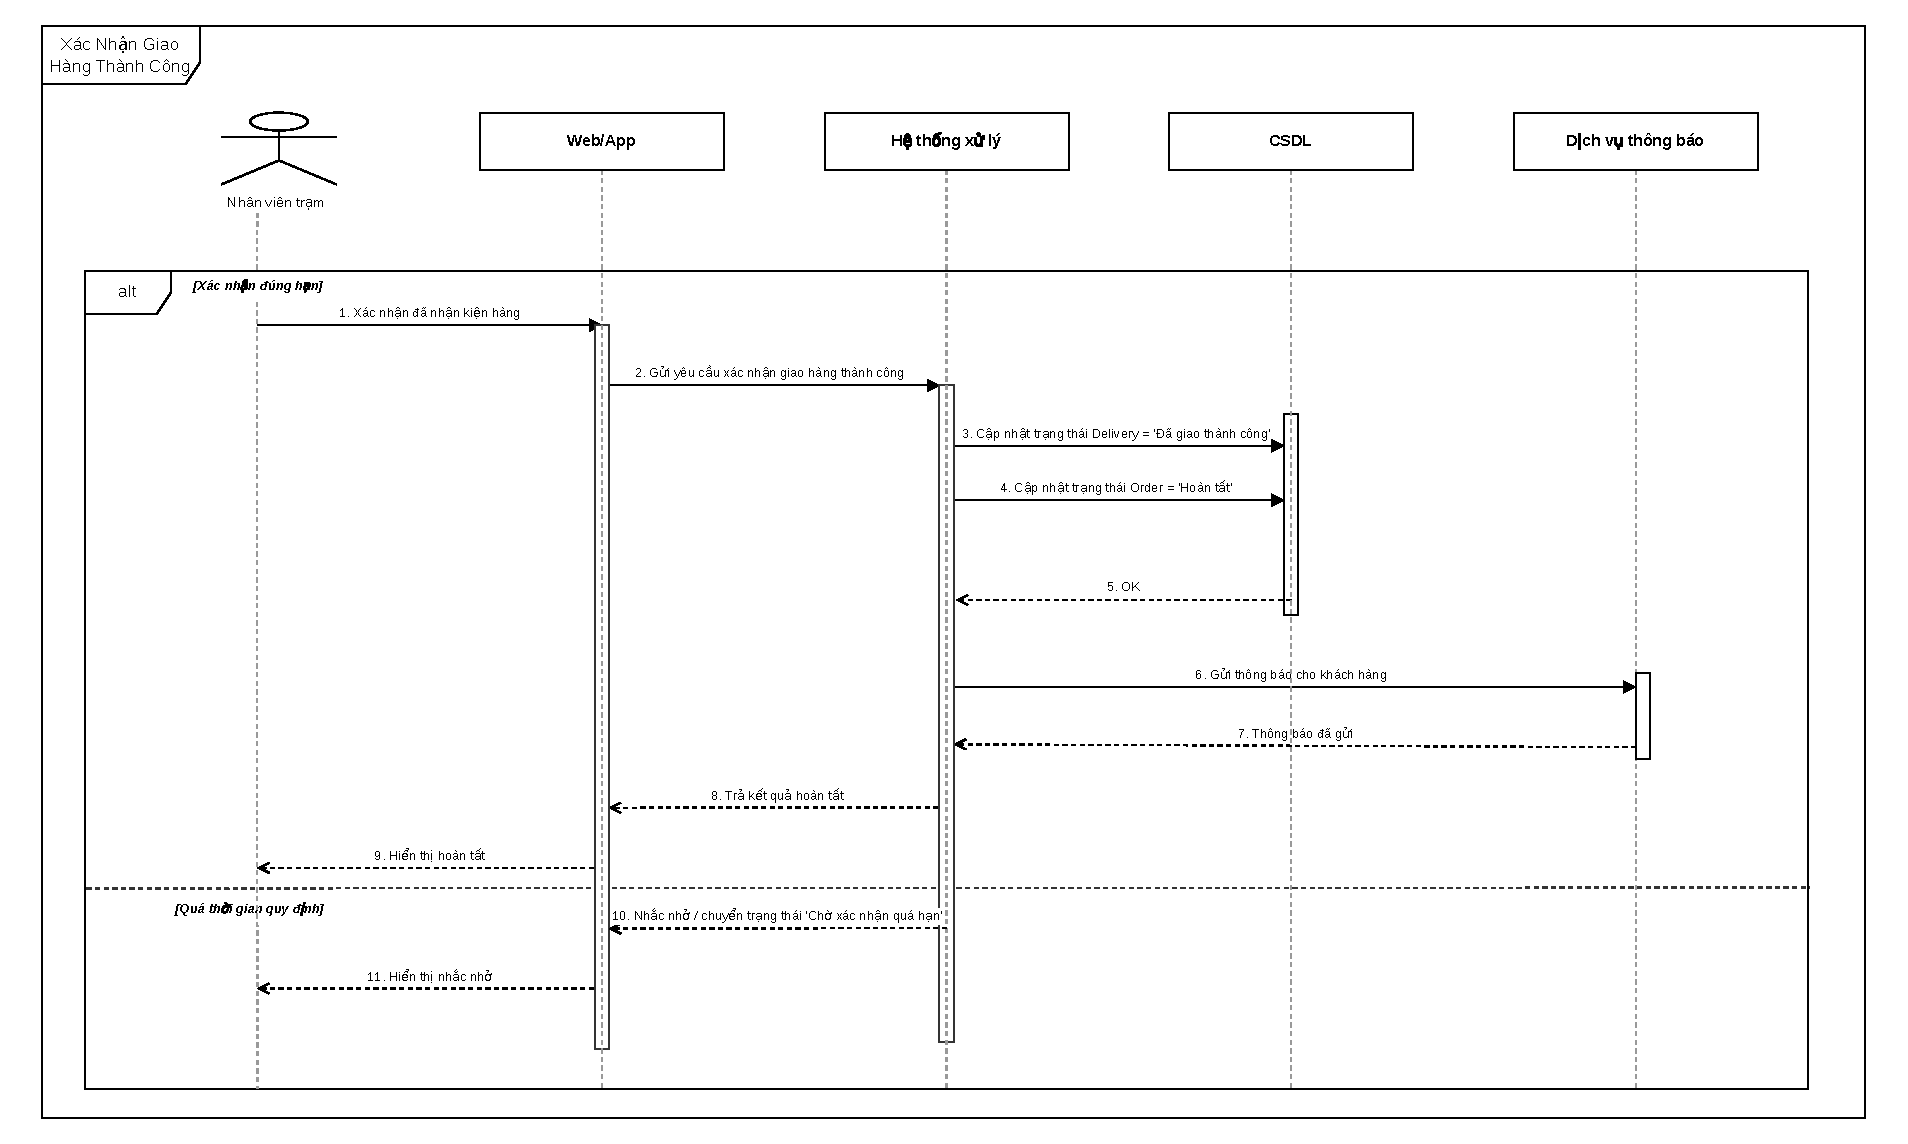
\includegraphics[width=\textwidth]{so-do/sodo-tuantu/Xác Nhận Giao Hàng Thành Công.drawio.pdf}
  \caption{Sơ đồ tuần tự chức năng Xác nhận giao hàng thành công}
  \label{fig:seq-uc09}
\end{figure}

\subsection{Ước Lượng Thời Gian Giao Hàng Dự Kiến}

\subsubsection{Sơ Đồ Lớp}
\begin{figure}[H]
  \centering
  
\includegraphics[width=0.85\textwidth]{diagrams/sodolop/UC10_UocLuongETA.png}
  \caption{Sơ đồ lớp chức năng Ước lượng thời gian giao hàng dự kiến (ETA)}
  \label{fig:class-uc10}
\end{figure}

\subsubsection{Đặc Tả Các Lớp}
\begin{table}[H]
  \centering
  \small
  \begin{tabularx}{\textwidth}{|c|>{\raggedright\arraybackslash}p{3.5cm}|>{\raggedright\arraybackslash}p{4.5cm}|>{\raggedright\arraybackslash}X|}
    \hline
    \textbf{STT} & \textbf{Tên lớp} & \textbf{Thuộc tính / Phương thức} & \textbf{Mô tả} \\
    \hline
    1 & \texttt{Dieu\allowbreak Khien\allowbreak Uoc\allowbreak Luong} & \texttt{lay\allowbreak Thoi\allowbreak Gian\allowbreak Du\allowbreak Kien\allowbreak (ma\allowbreak Don\allowbreak Hang)} & REST API controller tiếp nhận yêu cầu tính toán thời gian đến (ETA). \\ \hline
    2 & \texttt{Dich\allowbreak Vu\allowbreak Uoc\allowbreak Luong} & \texttt{tinh\allowbreak Thoi\allowbreak Gian\allowbreak Du\allowbreak Kien\allowbreak (ma\allowbreak Tram,\allowbreak ma\allowbreak Dia\allowbreak Chi)},\newline \texttt{- tinh\allowbreak Khoang\allowbreak Cach\allowbreak (vd1,\allowbreak kd1,\allowbreak vd2,\allowbreak kd2)} & Dịch vụ tính toán khoảng cách địa lý và quy đổi ra số phút bay ước lượng. \\ \hline
    3 & \texttt{Kho\allowbreak Du\allowbreak Lieu\allowbreak Tram\allowbreak Ha\allowbreak Canh} & \texttt{tim\allowbreak Theo\allowbreak Ma\allowbreak (ma)} & Interface Repository truy vấn thông tin tọa độ của trạm hạ cánh drone. \\ \hline
    4 & \texttt{Kho\allowbreak Du\allowbreak Lieu\allowbreak Dia\allowbreak Chi} & \texttt{tim\allowbreak Theo\allowbreak Ma\allowbreak (ma)} & Interface Repository truy vấn tọa độ điểm đến của khách hàng. \\ \hline
    5 & \texttt{Phan\allowbreak Hoi\allowbreak Uoc\allowbreak Luong} & \texttt{phut\allowbreak Du\allowbreak Kien}, \texttt{khoang\allowbreak Cach\allowbreak Km} & DTO đóng gói thời gian dự kiến (phút) và khoảng cách địa lý (km). \\ \hline
    6 & \texttt{Tram\allowbreak Ha\allowbreak Canh} & \texttt{ma\allowbreak Tram}, \texttt{vi\allowbreak Do}, \texttt{kinh\allowbreak Do} & Thực thể trạm hạ cánh chứa thông tin vị trí địa lý cố định. \\ \hline
    7 & \texttt{Dia\allowbreak Chi} & \texttt{ma\allowbreak Dia\allowbreak Chi}, \texttt{vi\allowbreak Do}, \texttt{kinh\allowbreak Do} & Thực thể địa chỉ khách hàng chứa thông tin tọa độ đích đến. \\
    \hline
  \end{tabularx}
  \caption{Đặc tả các lớp chức năng Ước Lượng Thời Gian Giao Hàng Dự Kiến}
  \label{tab:class-spec-uc10}
\end{table}

\subsection{Trợ Lý AI Cho Khách Hàng (Chatbot)}

\subsubsection{Sơ Đồ Lớp}
\begin{figure}[H]
  \centering
  
\includegraphics[width=0.85\textwidth]{diagrams/sodolop/UC11_ChatbotAI.png}
  \caption{Sơ đồ lớp chức năng Trợ lý AI cho khách hàng (Chatbot)}
  \label{fig:class-uc11}
\end{figure}

\subsubsection{Đặc Tả Các Lớp}
\begin{table}[H]
  \centering
  \small
  \begin{tabularx}{\textwidth}{|c|>{\raggedright\arraybackslash}p{3.5cm}|>{\raggedright\arraybackslash}p{4.5cm}|>{\raggedright\arraybackslash}X|}
    \hline
    \textbf{STT} & \textbf{Tên lớp} & \textbf{Thuộc tính / Phương thức} & \textbf{Mô tả} \\
    \hline
    1 & \texttt{Dieu\allowbreak Khien\allowbreak Tro\allowbreak Ly\allowbreak Hang} & \texttt{gui\allowbreak Cau\allowbreak Hoi\allowbreak (ma\allowbreak Kh,\allowbreak yeu\allowbreak Cau)} & REST API controller nhận nội dung tin nhắn gửi chatbot. \\ \hline
    2 & \texttt{Dich\allowbreak Vu\allowbreak Tro\allowbreak Ly\allowbreak Hang} & \texttt{tra\allowbreak Loi\allowbreak Cau\allowbreak Hoi\allowbreak (ma\allowbreak Kh,\allowbreak cau\allowbreak Hoi)},\newline \texttt{- tra\allowbreak Cuu\allowbreak Thong\allowbreak Tin\allowbreak Giao\allowbreak Hang\allowbreak (ma\allowbreak Kh)},\newline \texttt{- goi\allowbreak Dich\allowbreak Vu\allowbreak Mo\allowbreak Hinh\allowbreak Ngon\allowbreak Ngu\allowbreak (loi\allowbreak Nhac)} & Dịch vụ tập hợp ngữ cảnh đơn hàng của khách và gửi yêu cầu tới LLM API. \\ \hline
    3 & \texttt{Kho\allowbreak Du\allowbreak Lieu\allowbreak Tin\allowbreak Nhan\allowbreak Chatbot} & \texttt{luu\allowbreak (tin\allowbreak Nhan)} & Interface Repository lưu lịch sử trò chuyện vào CSDL. \\ \hline
    4 & \texttt{Kho\allowbreak Du\allowbreak Lieu\allowbreak Don\allowbreak Hang} & \texttt{tim\allowbreak Theo\allowbreak Ma\allowbreak Khach\allowbreak Hang\allowbreak (ma\allowbreak Kh)} & Interface Repository truy vấn thông tin đơn hàng hiện tại phục vụ làm context. \\ \hline
    5 & \texttt{Khach\allowbreak Hang\allowbreak Mo\allowbreak Hinh\allowbreak Ngon\allowbreak Ngu} & \texttt{tao\allowbreak Phan\allowbreak Hoi\allowbreak (loi\allowbreak Nhac)} & Interface giao tiếp với mô hình ngôn ngữ lớn bên ngoài (Gemini/Groq API). \\ \hline
    6 & \texttt{Yeu\allowbreak Cau\allowbreak Tro\allowbreak Chuyen} & \texttt{cau\allowbreak Hoi} & DTO đóng gói câu hỏi đầu vào của khách hàng gửi cho chatbot. \\ \hline
    7 & \texttt{Phan\allowbreak Hoi\allowbreak Tro\allowbreak Chuyen} & \texttt{tra\allowbreak Loi} & DTO chứa câu trả lời định dạng văn bản nhận được từ LLM. \\ \hline
    8 & \texttt{Tin\allowbreak Nhan\allowbreak Chatbot} & \texttt{ma\allowbreak Tin\allowbreak Nhan}, \texttt{noi\allowbreak Dung}, \texttt{phan\allowbreak Hoi} & Thực thể lưu trữ cặp câu hỏi - câu trả lời trong lịch sử chatbot. \\ \hline
    9 & \texttt{Don\allowbreak Hang} & \texttt{ma\allowbreak Don\allowbreak Hang}, \texttt{trang\allowbreak Thai} & Thực thể đơn hàng đóng vai trò làm dữ liệu ngữ cảnh cho chatbot. \\
    \hline
  \end{tabularx}
  \caption{Đặc tả các lớp chức năng Trợ Lý AI Cho Khách Hàng (Chatbot)}
  \label{tab:class-spec-uc11}
\end{table}

\subsection{Tạo và Quản Lý Tài Khoản Người Dùng}

\subsubsection{Sơ Đồ Lớp}
\begin{figure}[H]
  \centering
  
\includegraphics[width=0.85\textwidth]{diagrams/sodolop/UC12_QuanLyTaiKhoan.png}
  \caption{Sơ đồ lớp chức năng Tạo và quản lý tài khoản người dùng}
  \label{fig:class-uc12}
\end{figure}

\subsubsection{Đặc Tả Các Lớp}
\begin{table}[H]
  \centering
  \small
  \begin{tabularx}{\textwidth}{|c|>{\raggedright\arraybackslash}p{3.5cm}|>{\raggedright\arraybackslash}p{4.5cm}|>{\raggedright\arraybackslash}X|}
    \hline
    \textbf{STT} & \textbf{Tên lớp} & \textbf{Thuộc tính / Phương thức} & \textbf{Mô tả} \\
    \hline
    1 & \texttt{Dieu\allowbreak Khien\allowbreak Quan\allowbreak Ly\allowbreak Nguoi\allowbreak Dung} & \texttt{tao\allowbreak Nguoi\allowbreak Dung\allowbreak (yeu\allowbreak Cau)},\newline \texttt{cap\allowbreak Nhat\allowbreak Nguoi\allowbreak Dung\allowbreak (ma,\allowbreak yeu\allowbreak Cau)},\newline \texttt{khoa\allowbreak Nguoi\allowbreak Dung\allowbreak (ma)} & REST API controller tiếp nhận các tác vụ quản trị người dùng. \\ \hline
    2 & \texttt{Dich\allowbreak Vu\allowbreak Quan\allowbreak Ly\allowbreak Nguoi\allowbreak Dung} & \texttt{tao\allowbreak Nguoi\allowbreak Dung\allowbreak (yeu\allowbreak Cau)},\newline \texttt{cap\allowbreak Nhat\allowbreak Nguoi\allowbreak Dung\allowbreak (...)},\newline \texttt{- kiem\allowbreak Tra\allowbreak Thu\allowbreak Dien\allowbreak Tu\allowbreak Ton\allowbreak Tai\allowbreak (email)} & Dịch vụ xử lý logic quản lý người dùng, tạo tài khoản và phân quyền. \\ \hline
    3 & \texttt{Kho\allowbreak Du\allowbreak Lieu\allowbreak Nguoi\allowbreak Dung} & \texttt{luu\allowbreak (nguoi\allowbreak Dung)}, \texttt{tim\allowbreak Theo\allowbreak Thu\allowbreak Dien\allowbreak Tu\allowbreak (email)},\newline \texttt{tim\allowbreak Theo\allowbreak Ma\allowbreak (ma)} & Interface Repository lưu trữ dữ liệu người dùng thay đổi vào CSDL. \\ \hline
    4 & \texttt{Kho\allowbreak Du\allowbreak Lieu\allowbreak Vai\allowbreak Tro} & \texttt{tim\allowbreak Theo\allowbreak Ma\allowbreak (ma)} & Interface Repository truy xuất thông tin quyền hạn của vai trò. \\ \hline
    5 & \texttt{Yeu\allowbreak Cau\allowbreak Tao\allowbreak Nguoi\allowbreak Dung} & \texttt{ho\allowbreak Ten}, \texttt{thu\allowbreak Dien\allowbreak Tu}, \texttt{mat\allowbreak Khau}, \texttt{ma\allowbreak Vai\allowbreak Tro} & DTO chứa dữ liệu khai báo đăng ký người dùng mới. \\ \hline
    6 & \texttt{Yeu\allowbreak Cau\allowbreak Cap\allowbreak Nhat\allowbreak Nguoi\allowbreak Dung} & \texttt{ho\allowbreak Ten}, \texttt{ma\allowbreak Vai\allowbreak Tro} & DTO chứa các thông tin tài khoản cần cập nhật chỉnh sửa. \\ \hline
    7 & \texttt{Phan\allowbreak Hoi\allowbreak Nguoi\allowbreak Dung} & \texttt{ma\allowbreak Nguoi\allowbreak Dung}, \texttt{ho\allowbreak Ten}, \texttt{thu\allowbreak Dien\allowbreak Tu},\newline \texttt{ten\allowbreak Vai\allowbreak Tro} & DTO phản hồi kết quả chi tiết của người dùng được tác động thành công. \\ \hline
    8 & \texttt{Nguoi\allowbreak Dung} & \texttt{ma\allowbreak Nguoi\allowbreak Dung}, \texttt{ho\allowbreak Ten}, \texttt{thu\allowbreak Dien\allowbreak Tu} & Thực thể tài khoản của người dùng. \\ \hline
    9 & \texttt{Vai\allowbreak Tro} & \texttt{ma\allowbreak Vai\allowbreak Tro}, \texttt{ten\allowbreak Vai\allowbreak Tro} & Thực thể vai trò hệ thống gắn liền với tài khoản. \\
    \hline
  \end{tabularx}
  \caption{Đặc tả các lớp chức năng Tạo và Quản Lý Tài Khoản Người Dùng}
  \label{tab:class-spec-uc12}
\end{table}

\subsection{Quản Lý Thiết Bị Drone}

\subsubsection{Sơ Đồ Lớp}
\begin{figure}[H]
  \centering
  
\includegraphics[width=0.85\textwidth]{diagrams/sodolop/UC13_QuanLyDrone.png}
  \caption{Sơ đồ lớp chức năng Quản lý thiết bị Drone}
  \label{fig:class-uc13}
\end{figure}

\subsubsection{Đặc Tả Các Lớp}
\begin{table}[H]
  \centering
  \small
  \begin{tabularx}{\textwidth}{|c|>{\raggedright\arraybackslash}p{3.5cm}|>{\raggedright\arraybackslash}p{4.5cm}|>{\raggedright\arraybackslash}X|}
    \hline
    \textbf{STT} & \textbf{Tên lớp} & \textbf{Thuộc tính / Phương thức} & \textbf{Mô tả} \\
    \hline
    1 & \texttt{Dieu\allowbreak Khien\allowbreak Drone} & \texttt{lay\allowbreak Danh\allowbreak Sach\allowbreak Drone\allowbreak ()}, \texttt{tao\allowbreak Drone\allowbreak (yeu\allowbreak Cau)}, \texttt{cap\allowbreak Nhat\allowbreak Drone\allowbreak (ma,\allowbreak yeu\allowbreak Cau)}, \texttt{xoa\allowbreak Drone\allowbreak (ma)} & REST API controller tiếp nhận các tác vụ quản lý drone. \\ \hline
    2 & \texttt{Dich\allowbreak Vu\allowbreak Drone} & \texttt{lay\allowbreak Danh\allowbreak Sach\allowbreak Drone\allowbreak ()}, \texttt{tao\allowbreak Drone\allowbreak (yeu\allowbreak Cau)}, \texttt{cap\allowbreak Nhat\allowbreak Drone\allowbreak (...)},\newline \texttt{xoa\allowbreak Drone\allowbreak (ma)} & Lớp dịch vụ xử lý nghiệp vụ quản lý vòng đời drone và kiểm tra điều kiện ràng buộc trạng thái. \\ \hline
    3 & \texttt{Kho\allowbreak Du\allowbreak Lieu\allowbreak Drone} & \texttt{tim\allowbreak Tat\allowbreak Ca\allowbreak ()}, \texttt{tim\allowbreak Theo\allowbreak Ma\allowbreak (ma)}, \texttt{luu\allowbreak (drone)}, \texttt{xoa\allowbreak (ma)} & Interface Repository thực hiện các truy vấn dữ liệu thiết bị drone trong CSDL. \\ \hline
    4 & \texttt{Yeu\allowbreak Cau\allowbreak Tao\allowbreak Drone} & \texttt{trang\allowbreak Thai\allowbreak Drone}, \texttt{cong\allowbreak Suat\allowbreak Pin} & DTO đóng gói thông tin đăng ký drone mới. \\ \hline
    5 & \texttt{Yeu\allowbreak Cau\allowbreak Cap\allowbreak Nhat\allowbreak Drone} & \texttt{trang\allowbreak Thai\allowbreak Drone}, \texttt{cong\allowbreak Suat\allowbreak Pin}, \texttt{ngay\allowbreak Bao\allowbreak Tri\allowbreak Gan\allowbreak Nhat} & DTO đóng gói thông tin cập nhật cho thiết bị drone. \\ \hline
    6 & \texttt{Phan\allowbreak Hoi\allowbreak Drone} & \texttt{ma\allowbreak Drone}, \texttt{trang\allowbreak Thai\allowbreak Drone}, \texttt{cong\allowbreak Suat\allowbreak Pin}, \texttt{ngay\allowbreak Bao\allowbreak Tri\allowbreak Gan\allowbreak Nhat} & DTO phản hồi thông tin drone sau khi thực hiện tác vụ thành công. \\ \hline
    7 & \texttt{Drone} & \texttt{ma\allowbreak Drone}, \texttt{trang\allowbreak Thai\allowbreak Drone}, \texttt{cong\allowbreak Suat\allowbreak Pin}, \texttt{ngay\allowbreak Bao\allowbreak Tri\allowbreak Gan\allowbreak Nhat} & Thực thể biểu diễn thông tin drone trong CSDL. \\
    \hline
  \end{tabularx}
  \caption{Đặc tả các lớp chức năng Quản Lý Thiết Bị Drone}
  \label{tab:class-spec-uc13}
\end{table}

\subsubsection{Sơ Đồ Tuần Tự}
\begin{figure}[H]
  \centering
  \includegraphics[width=\textwidth]{so-do/sodo-tuantu/Quản lý thiết bị Drone.png}
  \caption{Sơ đồ tuần tự chức năng Quản lý thiết bị Drone}
  \label{fig:seq-uc13}
\end{figure}
